% ======================================================================
% IEEE Conference Paper -- Hardware-Focused
% FPGA-Based Quantized CNN Accelerators with Dynamic Activation Gating
% ======================================================================
\documentclass[conference]{IEEEtran}
\usepackage[utf8]{inputenc}
\usepackage{amsmath,amssymb,amsfonts}
\usepackage{algorithm}
\usepackage{algorithmic}
\usepackage{graphicx}
\usepackage{textcomp}
\usepackage{xcolor}
\usepackage{booktabs}
\usepackage{multirow}
\usepackage{float}
\usepackage{caption}
\usepackage{subcaption}
\usepackage{hyperref}
\usepackage{cite}
\usepackage{array}
\usepackage{balance}
\usepackage{enumitem}
\usepackage{tikz}
\usetikzlibrary{arrows.meta,positioning,calc,shapes.geometric,fit,decorations.pathreplacing}

\hypersetup{
    colorlinks=true,
    linkcolor=blue,
    citecolor=blue,
    urlcolor=blue
}

\begin{document}

\title{FPGA-Based Quantized CNN Accelerators with Dynamic Activation Gating: A Hardware Co-Design Study on Zynq-7020}

\author{
\IEEEauthorblockN{Hardware-AI Co-Design Group}
\IEEEauthorblockA{Department of Electronics and Communication Engineering}
}

\maketitle

% ======================================================================
\begin{abstract}
We present a hardware-software co-design study of Convolutional Neural Network (CNN) accelerators targeting the Xilinx Zynq-7020 FPGA. Three progressive RTL-level optimizations are systematically evaluated: Trained Ternary Quantization (TTQ) with folded Batch Normalization replaces per-tap DSP multipliers with ternary add/subtract logic, achieving $16\times$ weight compression. Density-Adaptive Activation Pruning (DAAP) introduces a 2-tap lookahead FSM that dynamically skips zero and sub-threshold activations, reducing CIFAR-10 inference cycles by 29.9\%. Spatial Hysteresis Gating extends this with 4-cardinal neighbor voting to create contiguous zero-clusters, achieving a $1.95\times$ speedup at the cost of 67.3\% LUT utilization. All eight accelerator variants (four per dataset: MNIST and CIFAR-10) are implemented in SystemVerilog, verified end-to-end in Vivado XSim, and synthesized on silicon with timing closure at 100~MHz (MNIST) and 40~MHz (CIFAR-10). The designs operate at ultra-low power ($<$200~mW), demonstrating feasibility for edge deployment in autonomous systems and IoT nodes.
\end{abstract}

\begin{IEEEkeywords}
FPGA, CNN accelerator, Ternary Quantization, Activation Pruning, Edge AI, Zynq-7020, Hardware-Software Co-Design, FSM, Lookahead Gating
\end{IEEEkeywords}


% ======================================================================
\section{Introduction}
\label{sec:introduction}
% ======================================================================

The deployment of Convolutional Neural Networks (CNNs) on edge devices demands inference engines that simultaneously satisfy strict constraints on latency, power, silicon area, and accuracy. While GPUs and dedicated ASICs dominate cloud-scale inference, Field Programmable Gate Arrays (FPGAs) offer a compelling alternative for edge deployment due to their reconfigurability, deterministic latency, and ultra-low power profiles~\cite{guo2019}.

FPGA-based CNN acceleration faces three fundamental hardware bottlenecks:

\begin{enumerate}[nosep]
    \item \textbf{Memory Wall}: Full-precision (FP32) weights require expensive off-chip DRAM access. On a Zynq-7020, storing a 120K-parameter model in FP32 consumes 48 of 140 BRAM36 tiles (34.3\%), leaving insufficient resources for activation buffering.
    \item \textbf{DSP Scarcity}: Each $32\times32$-bit signed multiplication requires 4 DSP48E1 slices on Xilinx 7-series devices~\cite{xilinx_zynq}. Parallelizing convolution with 4 filters per group consumes 88 of 220 DSPs (40\%) in a full-precision baseline.
    \item \textbf{Wasted Cycles}: Standard sequential accelerators execute one MAC per clock, unconditionally processing every activation-weight pair -- even when ReLU produces zero-valued activations (up to 73.7\% in deeper layers).
\end{enumerate}

Prior work on FPGA CNN accelerators has addressed these challenges individually. FINN~\cite{umuroglu2017,blott2018} demonstrated streaming dataflow architectures for binarized networks but requires framework-level integration. Mixed-precision approaches~\cite{wang2019,sharma2018} achieve flexibility but introduce complex control logic for heterogeneous precision across layers. Recent work on hardware-aware pruning~\cite{han2016,guo2017} shows promise but typically targets unstructured sparsity, which maps poorly to regular FPGA datapaths.

Our work differs from prior approaches in three key ways:

\begin{itemize}[nosep]
    \item \textbf{Integrated Co-Design}: We jointly optimize quantization (TTQ), activation pruning (DAAP), and spatial gating (Hysteresis) within a unified RTL pipeline FSM, rather than treating them as independent optimizations.
    \item \textbf{Skip-Gating FSM}: We introduce a lookahead FSM that exploits activation sparsity at the hardware level by advancing loop counters combinationally, achieving clock-cycle savings without pipeline stalls. Prior work~\cite{han2016,albericio2016} relies on compressed sparse formats that require decompression overhead.
    \item \textbf{Data-Dependent Analysis}: We provide the first direct comparison of magnitude-based (DAAP) vs. spatial (Hysteresis) activation gating across datasets with fundamentally different sparsity profiles (MNIST vs. CIFAR-10), revealing critical data-dependent limitations.
\end{itemize}

This paper is organized as follows: Section~\ref{sec:related} reviews related work. Section~\ref{sec:architecture} presents the network and hardware architectures. Section~\ref{sec:hw_design} details the RTL-level hardware design. Section~\ref{sec:results} provides experimental results. Section~\ref{sec:conclusion} concludes with future work.


% ======================================================================
\section{Related Work}
\label{sec:related}
% ======================================================================

\subsection{Weight Quantization for FPGA Inference}

Weight quantization reduces the bit-width of network parameters to lower memory and computation costs. Courbariaux et al.~\cite{courbariaux2016} introduced Binarized Neural Networks (BNNs) with 1-bit weights, achieving maximal compression but with significant accuracy loss on complex datasets. Li and Liu~\cite{li2016} proposed Ternary Weight Networks (TWNs) using a symmetric scale factor, while Zhu et al.~\cite{zhu2017} improved upon this with Trained Ternary Quantization (TTQ), introducing asymmetric learnable scales $W_p$ and $W_n$ that preserve representational capacity. Our hardware implementation builds upon TTQ by fusing the asymmetric scaling with folded Batch Normalization into a dedicated FSM stage, reducing the per-output-position overhead to a single multiply-add in hardware.

Jacob et al.~\cite{jacob2018} demonstrated 8-bit integer quantization for mobile deployment, while recent work by Nagel et al.~\cite{nagel2021} explored data-free quantization. However, these approaches still require DSP multipliers for each MAC tap. Our ternary approach eliminates all per-tap multipliers, replacing them with conditional add/subtract operations implemented purely in LUT fabric.

\subsection{FPGA CNN Accelerator Architectures}

The FINN framework~\cite{umuroglu2017,blott2018} pioneered streaming dataflow architectures for quantized neural networks on FPGAs, achieving high throughput through layer-wise pipeline parallelism. However, FINN targets binarized networks and requires HLS-based code generation. Venieris and Bouganis~\cite{venieris2018} proposed fpgaConvNet for automated mapping of CNNs to FPGAs, focusing on resource-performance trade-offs.

Sharma et al.~\cite{sharma2018} presented a bit-flexible accelerator supporting mixed-precision computation, while Qiu et al.~\cite{qiu2016} demonstrated a complete CNN accelerator on Zynq with dynamic fixed-point optimization. Our work extends the sequential pipeline FSM paradigm used in these designs by introducing skip-gating logic that exploits runtime activation sparsity -- a dimension largely unexplored in existing FPGA accelerator architectures.

\subsection{Activation Sparsity Exploitation}

Albericio et al.~\cite{albericio2016} proposed Cnvlutin, which skips zero-valued activations in GPU architectures using compressed representations. Han et al.~\cite{han2016} demonstrated Deep Compression combining pruning, quantization, and Huffman coding, but the resulting irregular sparsity patterns create memory access inefficiencies on FPGAs.

Recent hardware-aware approaches~\cite{zhang2022,chen2019} prune entire filters or channels (structured pruning) to maintain regular data flow, but sacrifice granularity. Our DAAP approach is complementary: it operates at the activation level (finer granularity than filter pruning) while maintaining regular FPGA data flow through the lookahead FSM skip mechanism. The spatial hysteresis extension further improves skip efficiency by clustering zero activations spatially, creating opportunities for multi-tap skipping that unstructured approaches cannot exploit.

\subsection{Gaps Addressed by This Work}

Existing literature lacks a unified FPGA accelerator that combines ternary quantization with runtime activation gating in a single RTL pipeline. Furthermore, no prior work compares magnitude-based and spatial activation gating strategies across datasets with different sparsity characteristics. Our co-design approach addresses both gaps, providing hardware-verified results on physical silicon rather than simulation-only estimates.


% ======================================================================
\section{System Architecture}
\label{sec:architecture}
% ======================================================================

\subsection{CNN Architectures}

We evaluate two CNN architectures of increasing complexity:

% --- MNIST Architecture Flowchart ---
\begin{figure}[H]
\centering
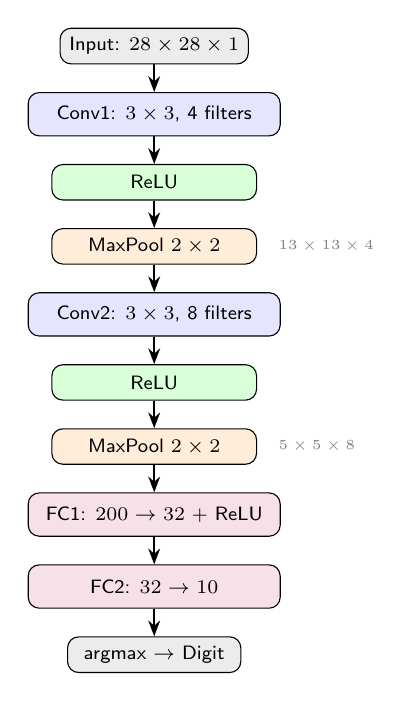
\begin{tikzpicture}[
    node distance=0.35cm,
    block/.style={draw, rounded corners, fill=blue!10, minimum width=3.2cm,
                  minimum height=0.55cm, font=\scriptsize\sffamily, align=center},
    act/.style={draw, rounded corners, fill=green!15, minimum width=2.6cm,
                minimum height=0.45cm, font=\scriptsize\sffamily},
    pool/.style={draw, rounded corners, fill=orange!15, minimum width=2.6cm,
                 minimum height=0.45cm, font=\scriptsize\sffamily},
    fc/.style={draw, rounded corners, fill=purple!12, minimum width=3.2cm,
               minimum height=0.55cm, font=\scriptsize\sffamily, align=center},
    io/.style={draw, rounded corners, fill=gray!15, minimum width=2.2cm,
               minimum height=0.45cm, font=\scriptsize\sffamily},
    arr/.style={-{Stealth[length=2mm]}, thick},
    dim/.style={font=\tiny\sffamily, text=gray}
]
    \node[io] (in) {Input: $28\times28\times1$};
    \node[block, below=of in] (c1) {Conv1: $3\times3$, 4 filters};
    \node[act, below=of c1] (r1) {ReLU};
    \node[pool, below=of r1] (p1) {MaxPool $2\times2$};
    \node[dim, right=0.15cm of p1] {$13\times13\times4$};
    \node[block, below=of p1] (c2) {Conv2: $3\times3$, 8 filters};
    \node[act, below=of c2] (r2) {ReLU};
    \node[pool, below=of r2] (p2) {MaxPool $2\times2$};
    \node[dim, right=0.15cm of p2] {$5\times5\times8$};
    \node[fc, below=of p2] (fc1) {FC1: $200 \to 32$ + ReLU};
    \node[fc, below=of fc1] (fc2) {FC2: $32 \to 10$};
    \node[io, below=of fc2] (out) {argmax $\to$ Digit};
    
    \draw[arr] (in) -- (c1);
    \draw[arr] (c1) -- (r1);
    \draw[arr] (r1) -- (p1);
    \draw[arr] (p1) -- (c2);
    \draw[arr] (c2) -- (r2);
    \draw[arr] (r2) -- (p2);
    \draw[arr] (p2) -- (fc1);
    \draw[arr] (fc1) -- (fc2);
    \draw[arr] (fc2) -- (out);
\end{tikzpicture}
\caption{MNIST CNN architecture (7,098 parameters).}
\label{fig:mnist_arch}
\end{figure}

% --- CIFAR-10 Architecture Flowchart ---
\begin{figure}[H]
\centering
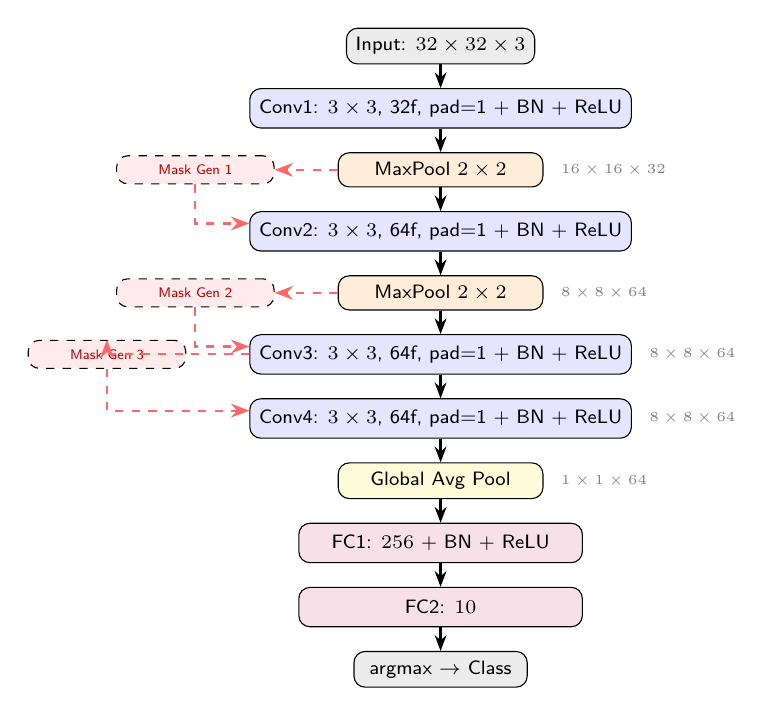
\begin{tikzpicture}[
    node distance=0.3cm,
    block/.style={draw, rounded corners, fill=blue!10, minimum width=3.6cm,
                  minimum height=0.5cm, font=\scriptsize\sffamily, align=center},
    act/.style={draw, rounded corners, fill=green!15, minimum width=2.6cm,
                minimum height=0.4cm, font=\scriptsize\sffamily},
    pool/.style={draw, rounded corners, fill=orange!15, minimum width=2.6cm,
                 minimum height=0.4cm, font=\scriptsize\sffamily},
    fc/.style={draw, rounded corners, fill=purple!12, minimum width=3.6cm,
               minimum height=0.5cm, font=\scriptsize\sffamily, align=center},
    gap/.style={draw, rounded corners, fill=yellow!15, minimum width=2.6cm,
                minimum height=0.4cm, font=\scriptsize\sffamily},
    io/.style={draw, rounded corners, fill=gray!15, minimum width=2.2cm,
               minimum height=0.4cm, font=\scriptsize\sffamily},
    arr/.style={-{Stealth[length=2mm]}, thick},
    dim/.style={font=\tiny\sffamily, text=gray},
    mask/.style={draw, dashed, rounded corners, fill=red!8, minimum width=2.0cm,
                 minimum height=0.35cm, font=\tiny\sffamily, text=red!70!black}
]
    \node[io] (in) {Input: $32\times32\times3$};
    \node[block, below=of in] (c1) {Conv1: $3\times3$, 32f, pad=1 + BN + ReLU};
    \node[pool, below=of c1] (p1) {MaxPool $2\times2$};
    \node[dim, right=0.1cm of p1] {$16\times16\times32$};
    \node[mask, left=0.8cm of p1] (m1) {Mask Gen 1};
    
    \node[block, below=of p1] (c2) {Conv2: $3\times3$, 64f, pad=1 + BN + ReLU};
    \node[pool, below=of c2] (p2) {MaxPool $2\times2$};
    \node[dim, right=0.1cm of p2] {$8\times8\times64$};
    \node[mask, left=0.8cm of p2] (m2) {Mask Gen 2};
    
    \node[block, below=of p2] (c3) {Conv3: $3\times3$, 64f, pad=1 + BN + ReLU};
    \node[dim, right=0.1cm of c3] {$8\times8\times64$};
    \node[mask, left=0.8cm of c3] (m3) {Mask Gen 3};
    
    \node[block, below=of c3] (c4) {Conv4: $3\times3$, 64f, pad=1 + BN + ReLU};
    \node[dim, right=0.1cm of c4] {$8\times8\times64$};
    
    \node[gap, below=of c4] (g) {Global Avg Pool};
    \node[dim, right=0.1cm of g] {$1\times1\times64$};
    \node[fc, below=of g] (fc1) {FC1: $256$ + BN + ReLU};
    \node[fc, below=of fc1] (fc2) {FC2: $10$};
    \node[io, below=of fc2] (out) {argmax $\to$ Class};
    
    \draw[arr] (in) -- (c1);
    \draw[arr] (c1) -- (p1);
    \draw[arr] (p1) -- (c2);
    \draw[arr] (c2) -- (p2);
    \draw[arr] (p2) -- (c3);
    \draw[arr] (c3) -- (c4);
    \draw[arr] (c4) -- (g);
    \draw[arr] (g) -- (fc1);
    \draw[arr] (fc1) -- (fc2);
    \draw[arr] (fc2) -- (out);
    
    \draw[-{Stealth}, dashed, red!60, thick] (p1.west) -- (m1.east);
    \draw[-{Stealth}, dashed, red!60, thick] (m1.south) |- ([yshift=0.1cm]c2.west);
    \draw[-{Stealth}, dashed, red!60, thick] (p2.west) -- (m2.east);
    \draw[-{Stealth}, dashed, red!60, thick] (m2.south) |- ([yshift=0.1cm]c3.west);
    \draw[-{Stealth}, dashed, red!60, thick] (c3.west) -| (m3.north);
    \draw[-{Stealth}, dashed, red!60, thick] (m3.south) |- ([yshift=0.1cm]c4.west);
\end{tikzpicture}
\caption{CIFAR-10 CNN architecture (120,490 parameters). Dashed red lines show activation mask flow for pruning/hysteresis variants.}
\label{fig:cifar_arch}
\end{figure}

\subsection{Hardware Pipeline Block Diagram}

All accelerator variants share a unified sequential pipeline FSM, depicted in Fig.~\ref{fig:hw_pipeline}. The pipeline processes one layer at a time, reading activations from one feature-map buffer and writing results to the other in a ping-pong fashion. Under TTQ, the convolution MAC is replaced by ternary accumulation (add/subtract/skip) with dedicated SCALE and BN stages. The activation mask generator (present only in threshold/hysteresis variants) produces a skip mask consumed by the lookahead FSM in the subsequent layer.

\begin{figure*}[t]
\centering
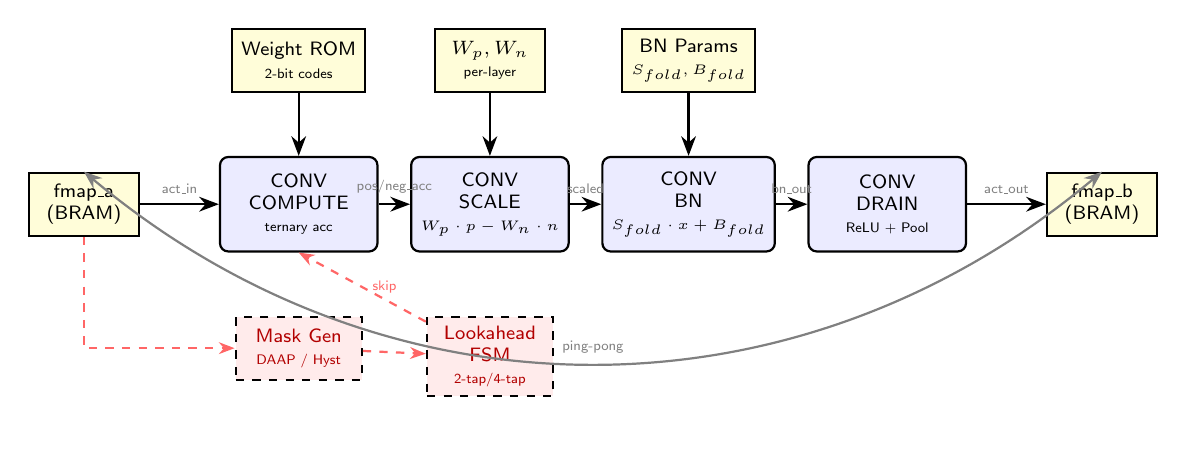
\begin{tikzpicture}[
    node distance=0.6cm and 0.4cm,
    stage/.style={draw, thick, rounded corners=3pt, fill=blue!8,
                  minimum width=2.0cm, minimum height=1.2cm,
                  font=\scriptsize\sffamily, align=center},
    mem/.style={draw, thick, fill=yellow!15, minimum width=1.4cm,
                minimum height=0.8cm, font=\scriptsize\sffamily, align=center},
    ctrl/.style={draw, thick, dashed, fill=red!8, minimum width=1.6cm,
                 minimum height=0.8cm, font=\scriptsize\sffamily, align=center,
                 text=red!70!black},
    arr/.style={-{Stealth[length=2.5mm]}, thick},
    darr/.style={-{Stealth[length=2mm]}, thick, dashed, red!60},
    lbl/.style={font=\tiny\sffamily, text=gray}
]
    % Memory
    \node[mem] (fmapA) {fmap\_a\\(BRAM)};
    
    % Conv pipeline stages
    \node[stage, right=1.0cm of fmapA] (compute) {CONV\\COMPUTE\\{\tiny ternary acc}};
    \node[stage, right=of compute] (scale) {CONV\\SCALE\\{\tiny $W_p \cdot p - W_n \cdot n$}};
    \node[stage, right=of scale] (bn) {CONV\\BN\\{\tiny $S_{fold}\cdot x + B_{fold}$}};
    \node[stage, right=of bn] (drain) {CONV\\DRAIN\\{\tiny ReLU + Pool}};
    
    \node[mem, right=1.0cm of drain] (fmapB) {fmap\_b\\(BRAM)};
    
    % Weight memory
    \node[mem, above=0.8cm of compute] (wrom) {Weight ROM\\{\tiny 2-bit codes}};
    
    % Mask generator
    \node[ctrl, below=0.8cm of compute] (mask) {Mask Gen\\{\tiny DAAP / Hyst}};
    
    % Lookahead FSM
    \node[ctrl, below=0.8cm of scale] (lookahead) {Lookahead\\FSM\\{\tiny 2-tap/4-tap}};
    
    % BN params
    \node[mem, above=0.8cm of bn] (bnparam) {BN Params\\{\tiny $S_{fold}, B_{fold}$}};
    
    % Scale params
    \node[mem, above=0.8cm of scale] (wpwn) {$W_p, W_n$\\{\tiny per-layer}};
    
    % Arrows
    \draw[arr] (fmapA) -- node[above, lbl] {act\_in} (compute);
    \draw[arr] (compute) -- node[above, lbl] {pos/neg\_acc} (scale);
    \draw[arr] (scale) -- node[above, lbl] {scaled} (bn);
    \draw[arr] (bn) -- node[above, lbl] {bn\_out} (drain);
    \draw[arr] (drain) -- node[above, lbl] {act\_out} (fmapB);
    
    \draw[arr] (wrom) -- (compute);
    \draw[arr] (wpwn) -- (scale);
    \draw[arr] (bnparam) -- (bn);
    
    \draw[darr] (fmapA.south) |- (mask);
    \draw[darr] (mask) -- (lookahead);
    \draw[darr] (lookahead) -- node[right, lbl, text=red!60] {skip} (compute.south);
    
    % Ping-pong annotation
    \draw[{Stealth}-{Stealth}, gray, thick] (fmapB.north) to[bend left=40]
        node[above, font=\tiny\sffamily, text=gray] {ping-pong} (fmapA.north);
    
\end{tikzpicture}
\caption{Hardware pipeline block diagram for TTQ+BN accelerator with optional activation gating. The dashed red path shows the mask generation and lookahead skip logic (active only in threshold/hysteresis variants).}
\label{fig:hw_pipeline}
\end{figure*}


% ======================================================================
\section{Hardware Design}
\label{sec:hw_design}
% ======================================================================

\subsection{Q16.16 Fixed-Point Datapath}

All activations, biases, BN parameters, and intermediate accumulators use Q16.16 signed fixed-point: 1 sign bit, 15 integer bits, 16 fractional bits. Range: $[-32768.0, +32767.99998]$, resolution: $2^{-16} \approx 1.53 \times 10^{-5}$. Multiplication produces a 64-bit product, right-shifted by 16 to return to Q16.16.

\subsection{Trained Ternary Quantization (TTQ) Hardware}

TTQ~\cite{zhu2017} quantizes each weight to $\{-W_n, 0, +W_p\}$ using asymmetric learnable scale factors. The quantization rule during training is:
\begin{equation}
W_q = \begin{cases}
    +W_p & \text{if } W > \Delta \\
    0 & \text{if } -\Delta \leq W \leq \Delta \\
    -W_n & \text{if } W < -\Delta
\end{cases}
\label{eq:ttq}
\end{equation}
where $\Delta = 0.05 \times \max(|W|)$. The scale factors are updated via gradient accumulation~\cite{zhu2017}:
\begin{equation}
\frac{\partial L}{\partial W_p} = \sum_{i \in S^+} \frac{\partial L}{\partial W_{q,i}}, \quad
\frac{\partial L}{\partial W_n} = \sum_{i \in S^-} -\frac{\partial L}{\partial W_{q,i}}
\end{equation}

Each weight is stored as a 2-bit code ($00$=zero, $01$=positive, $10$=negative), achieving $16\times$ compression over FP32. The hardware convolution pipeline (Algorithm~\ref{alg:ttq_conv}) replaces DSP multipliers with conditional add/subtract logic.

\begin{algorithm}[H]
\caption{TTQ Convolution Pipeline (Single Output Position)}
\label{alg:ttq_conv}
\begin{algorithmic}[1]
\STATE \textbf{Input:} activation buffer $A[]$, ternary codes $W[]$, scales $W_p, W_n$, BN params $S_f, B_f$
\STATE $\text{pos\_acc} \gets 0$; $\text{neg\_acc} \gets 0$
\FOR{each tap index $t = 0$ \TO $\text{TAP\_COUNT}-1$}
    \STATE $\text{code} \gets W[t]$ \COMMENT{2-bit read}
    \IF{$\text{code} = 01$}
        \STATE $\text{pos\_acc} \gets \text{pos\_acc} + A[t]$
    \ELSIF{$\text{code} = 10$}
        \STATE $\text{neg\_acc} \gets \text{neg\_acc} + A[t]$
    \ENDIF
\ENDFOR
\STATE $\text{scaled} \gets W_p \cdot \text{pos\_acc} - W_n \cdot \text{neg\_acc}$ \COMMENT{2 DSP mults}
\STATE $\text{bn\_out} \gets S_f \cdot \text{scaled} + B_f$ \COMMENT{1 DSP mult}
\STATE $\text{output} \gets \max(0, \text{bn\_out})$ \COMMENT{ReLU}
\end{algorithmic}
\end{algorithm}

\textbf{Key Hardware Insight}: DSP slices are consumed only in Lines 11--12 (SCALE and BN stages), executed once per output position. The inner loop (Lines 3--10) uses zero DSPs, enabling the inner loop to be implemented entirely in LUT fabric. This fundamentally changes the DSP scaling law from $O(\text{parallelism})$ to $O(1)$ per module.

\subsection{Batch Normalization Folding}

BN parameters ($\gamma, \beta, \mu, \sigma^2$) are folded into precomputed per-channel constants during weight export:
\begin{equation}
S_{\text{fold}} = \frac{\gamma}{\sqrt{\sigma^2 + \epsilon}}, \quad B_{\text{fold}} = \beta - \frac{\gamma \cdot \mu}{\sqrt{\sigma^2 + \epsilon}}
\end{equation}

This eliminates division and square-root operations from hardware, reducing BN to a single multiply-add in a dedicated FSM state (\texttt{S\_CONV\_BN}).

\subsection{Density-Adaptive Activation Pruning (DAAP)}
\label{sec:daap}

DAAP exploits the observation that ReLU produces sparse activation maps (23.9--73.7\% zeros across layers). Rather than processing all activations unconditionally, DAAP introduces per-filter thresholds that gate low-magnitude activations.

\begin{algorithm}[H]
\caption{DAAP Threshold Computation and Gating}
\label{alg:daap}
\begin{algorithmic}[1]
\STATE \textbf{Offline Calibration:}
\FOR{each filter $f$}
    \STATE $\rho_f \gets \frac{\text{non-zero ternary codes in } f}{\text{total codes in } f}$ \COMMENT{weight density}
    \STATE $\tau_f \gets \frac{\tau_{\text{base}}}{\max(\rho_f, 0.01)}$ \COMMENT{inverse density scaling}
\ENDFOR
\STATE \textbf{Runtime Gating (Hardware):}
\FOR{each activation $x$ at tap index $t$}
    \IF{$|x| < \tau_{f}$ \OR $W[t] = 00$}
        \STATE \textbf{skip} (advance counter, no accumulate)
    \ELSE
        \STATE Execute ternary accumulate (Algorithm~\ref{alg:ttq_conv}, Lines 5--9)
    \ENDIF
\ENDFOR
\end{algorithmic}
\end{algorithm}

The inverse density scaling (Line 4) ensures that filters with sparser weights receive higher thresholds, since each non-zero weight contributes proportionally more to the output. $\tau_{\text{base}}$ is calibrated via a validation-set sweep (0.0--0.8 for MNIST, optimal at 0.30; 0.0--0.02 for CIFAR-10, optimal at 0.003).

\textbf{Hardware Implementation}: Thresholds are loaded into distributed registers at startup via \texttt{\$readmemh}. In \texttt{S\_CONV\_COMPUTE}, a combinational comparator evaluates the skip condition with zero latency overhead:
\begin{verbatim}
wire skip = (w_code == 2'b00) ||
            (|act_in| < thresh[filter_idx]);
\end{verbatim}

\subsection{Spatial Hysteresis Gating}
\label{sec:hysteresis}

Hysteresis gating extends DAAP by incorporating spatial context, exploiting the observation that informative activations cluster spatially while noise activations are isolated.

\begin{algorithm}[H]
\caption{Spatial Hysteresis Mask Generation}
\label{alg:hyst}
\begin{algorithmic}[1]
\STATE \textbf{Pass 1 -- Classification:}
\FOR{each position $i$ in activation map}
    \IF{$|A[i]| > T_H$}
        \STATE $\text{status}[i] \gets \text{ACTIVE}$
    \ELSIF{$|A[i]| < T_L$}
        \STATE $\text{status}[i] \gets \text{INACTIVE}$
    \ELSE
        \STATE $\text{status}[i] \gets \text{UNCERTAIN}$
    \ENDIF
\ENDFOR
\STATE \textbf{Pass 2 -- 4-Cardinal Neighbor Resolution:}
\FOR{each position $i$ where $\text{status}[i] = \text{UNCERTAIN}$}
    \STATE $N_{\text{active}} \gets$ count of ACTIVE neighbors (N, S, E, W)
    \IF{$N_{\text{active}} \geq 2$}
        \STATE $\text{mask}[i] \gets 1$ \COMMENT{keep activation}
    \ELSE
        \STATE $\text{mask}[i] \gets 0$ \COMMENT{prune activation}
    \ENDIF
\ENDFOR
\end{algorithmic}
\end{algorithm}

\textbf{Key Hardware Benefit}: By forcing isolated low-magnitude activations to zero, hysteresis creates contiguous spatial zero-clusters. When the lookahead FSM encounters these clusters, it skips multiple consecutive taps at once, dramatically improving skip efficiency compared to the scattered zero patterns produced by magnitude-only thresholding.

\textbf{v5 LUTRAM Optimization}: The initial implementation used flat register outputs (\texttt{mask\_out} at 8,192 bits), requiring a 13-level MUX tree ($\sim$8,000 LUTs per read). This caused a 224\% LUT utilization failure (119K LUTs). The v5 redesign replaced the flat output with write-only ports and localized distributed RAMs (LUTRAM) inside the consumer convolution modules, reducing mask generator LUT usage from 59,520 to 198 -- a 99.6\% reduction.

\subsection{Lookahead Skip-Gating FSM}
\label{sec:lookahead}

The lookahead FSM is the core hardware mechanism that translates activation sparsity into clock-cycle savings. When the skip condition is true (zero weight code or sub-threshold activation), the FSM advances the loop counter combinationally without executing an accumulate operation.

\begin{algorithm}[H]
\caption{2-Tap Lookahead FSM (Convolution Layers)}
\label{alg:lookahead}
\begin{algorithmic}[1]
\STATE \textbf{In state} \texttt{S\_CONV\_COMPUTE}:
\STATE $\text{skip}_0 \gets (W[\text{idx}] = 00)$ \OR $(|A[\text{idx}]| < \tau)$
\STATE $\text{skip}_1 \gets (W[\text{idx}+1] = 00)$ \OR $(|A[\text{idx}+1]| < \tau)$
\IF{$\text{skip}_0$ \AND $\text{skip}_1$}
    \STATE $\text{idx} \gets \text{idx} + 2$ \COMMENT{skip 2 taps in 1 cycle}
\ELSIF{$\text{skip}_0$}
    \STATE $\text{idx} \gets \text{idx} + 1$ \COMMENT{skip 1 tap}
\ELSE
    \STATE Execute ternary accumulate for tap $\text{idx}$
    \STATE $\text{idx} \gets \text{idx} + 1$
\ENDIF
\end{algorithmic}
\end{algorithm}

\textbf{FC layers use 4-tap lookahead} ($L=4$) because FC addressing is purely linear ($\text{idx}+1, +2, +3$), allowing 4 parallel comparisons within timing. In convolution layers, 4-tap lookahead was evaluated but rejected: the 2D address computation requires checking kernel column/row wrapping boundaries ($kc \geq \text{K\_W}-1$, $kr \geq \text{K\_H}-1$) and computing stride-dependent offsets. This produces $>$50 combinational logic levels, creating a critical path exceeding 14.5~ns -- violating the 10~ns target at 100~MHz.

\subsection{Memory Architecture}

\subsubsection{Feature Map Ping-Pong Buffering}
Two BRAM buffers (\texttt{fmap\_a}, \texttt{fmap\_b}) alternate between layers: Phase~0 reads \texttt{fmap\_a} and writes \texttt{fmap\_b}; Phase~1 reverses. This saves 7 BRAM36 tiles compared to per-layer dedicated buffers.

\subsubsection{Weight Storage under TTQ}
Under TTQ, 2-bit ternary codes replace 32-bit FP weights. For MNIST, weight BRAM drops from 9 to 1 tile ($9\times$ reduction). For CIFAR-10, it drops from 48 to 16 tiles ($3\times$ reduction), since 32 of the original 48 tiles stored FC1 weights in FP32.

\subsubsection{Weight Array Partitioning}
Monolithic multi-dimensional weight arrays cause LUT explosion when Vivado infers multi-port read logic instead of BRAM (Vivado requires $\leq$2 ports for BRAM inference). Partitioning into channel-specific 1D arrays enabled BRAM inference, reducing Conv3 LUT usage from 84,983 to 1,165 in the CIFAR-10 baseline.


% ======================================================================
\section{Experimental Results}
\label{sec:results}
% ======================================================================

All designs are implemented in SystemVerilog, verified end-to-end in Vivado XSim, and synthesized on the Xilinx Zynq-7020 (XC7Z020). MNIST designs target 100~MHz; CIFAR-10 designs target 40~MHz.

\subsection{Software Accuracy}

Table~\ref{tab:software_acc} reports classification accuracy across all configurations. The CIFAR-10 full-precision baseline achieves 91.86\% using Knowledge Distillation (KD) from a larger teacher network.

\begin{table}[H]
\centering
\caption{Software Classification Accuracy}
\label{tab:software_acc}
\begin{tabular}{lcc}
\toprule
\textbf{Configuration} & \textbf{MNIST} & \textbf{CIFAR-10} \\
\midrule
Full-Precision Baseline & 98.35\% & 91.86\% \\
TTQ + BN & 97.28\% & 90.62\% \\
TTQ + BN + Threshold & 97.25\% & 89.85\% \\
TTQ + BN + Hysteresis & 96.96\% & 88.34\% \\
\midrule
$\Delta$ (TTQ vs Baseline) & $-1.07\%$ & $-1.24\%$ \\
$\Delta$ (Threshold vs TTQ) & $-0.03\%$ & $-0.77\%$ \\
$\Delta$ (Hysteresis vs TTQ) & $-0.32\%$ & $-2.28\%$ \\
\bottomrule
\end{tabular}
\end{table}

\textbf{Observations}: TTQ loses 1.24\% on CIFAR-10 due to the coarse ternary approximation of weights in a complex natural-image classification task. DAAP adds only $-0.77\%$, confirming that near-zero activations contribute negligibly. Hysteresis costs $-2.28\%$ on CIFAR-10 because the 4-cardinal neighbor voting assumes spatial locality -- an assumption violated by dense, texture-rich activation maps.

\subsection{Master Hardware Comparison}

Table~\ref{tab:master} presents the complete hardware metrics for all eight configurations.

\begin{table*}[t]
\centering
\caption{Hardware Implementation Metrics on Zynq-7020}
\label{tab:master}
\resizebox{\textwidth}{!}{
\begin{tabular}{lccccccccc}
\toprule
\textbf{Design} & \textbf{Dataset} & \textbf{Accuracy} & \textbf{Cycles} & \textbf{Latency} & \textbf{LUTs (\%)} & \textbf{FFs (\%)} & \textbf{BRAMs (\%)} & \textbf{DSPs (\%)} & \textbf{Power (W)} \\
\midrule
1. Sequential Baseline & MNIST & 98.35\% & 83,198 & 0.832 ms & 14,925 (28.1\%) & 31,571 (29.7\%) & 9 (6.4\%) & 23 (10.5\%) & 0.161 \\
2. TTQ + BN & MNIST & 97.28\% & 90,534 & 0.905 ms & 14,588 (27.4\%) & 31,523 (29.6\%) & 1 (0.7\%) & 51 (23.2\%) & 0.153 \\
3. TTQ + Threshold & MNIST & 97.25\% & 88,706 & 0.887 ms & 23,085 (43.4\%) & 31,591 (29.7\%) & 1 (0.7\%) & 54 (24.6\%) & 0.171 \\
4. TTQ + Hysteresis & MNIST & 96.96\% & 81,505 & 0.815 ms & 33,565 (63.1\%) & 32,734 (30.8\%) & 1 (0.7\%) & 54 (24.6\%) & 0.200 \\
\midrule
5. Full KD Baseline & CIFAR-10 & 91.86\% & 2,820,156 & 70.50 ms & 23,241 (43.7\%) & 15,632 (14.7\%) & 48 (34.3\%) & 88 (40.0\%) & 0.182 \\
6. TTQ + BN & CIFAR-10 & 90.62\% & 2,877,770 & 71.94 ms & 24,689 (46.4\%) & 16,437 (15.5\%) & 16 (11.4\%) & 36 (16.4\%) & 0.154 \\
7. TTQ + Threshold & CIFAR-10 & 89.85\% & 2,017,961 & 50.45 ms & 31,828 (59.8\%) & 16,769 (15.8\%) & 16 (11.4\%) & 36 (16.4\%) & 0.162 \\
8. TTQ + Hysteresis & CIFAR-10 & 88.34\% & 1,475,264 & 36.88 ms & 35,798 (67.3\%) & 16,623 (15.6\%) & 17.5 (12.5\%) & 36 (16.4\%) & 0.160 \\
\bottomrule
\end{tabular}
}
\end{table*}

\subsection{Resource Utilization Analysis}

\begin{figure}[H]
\centering
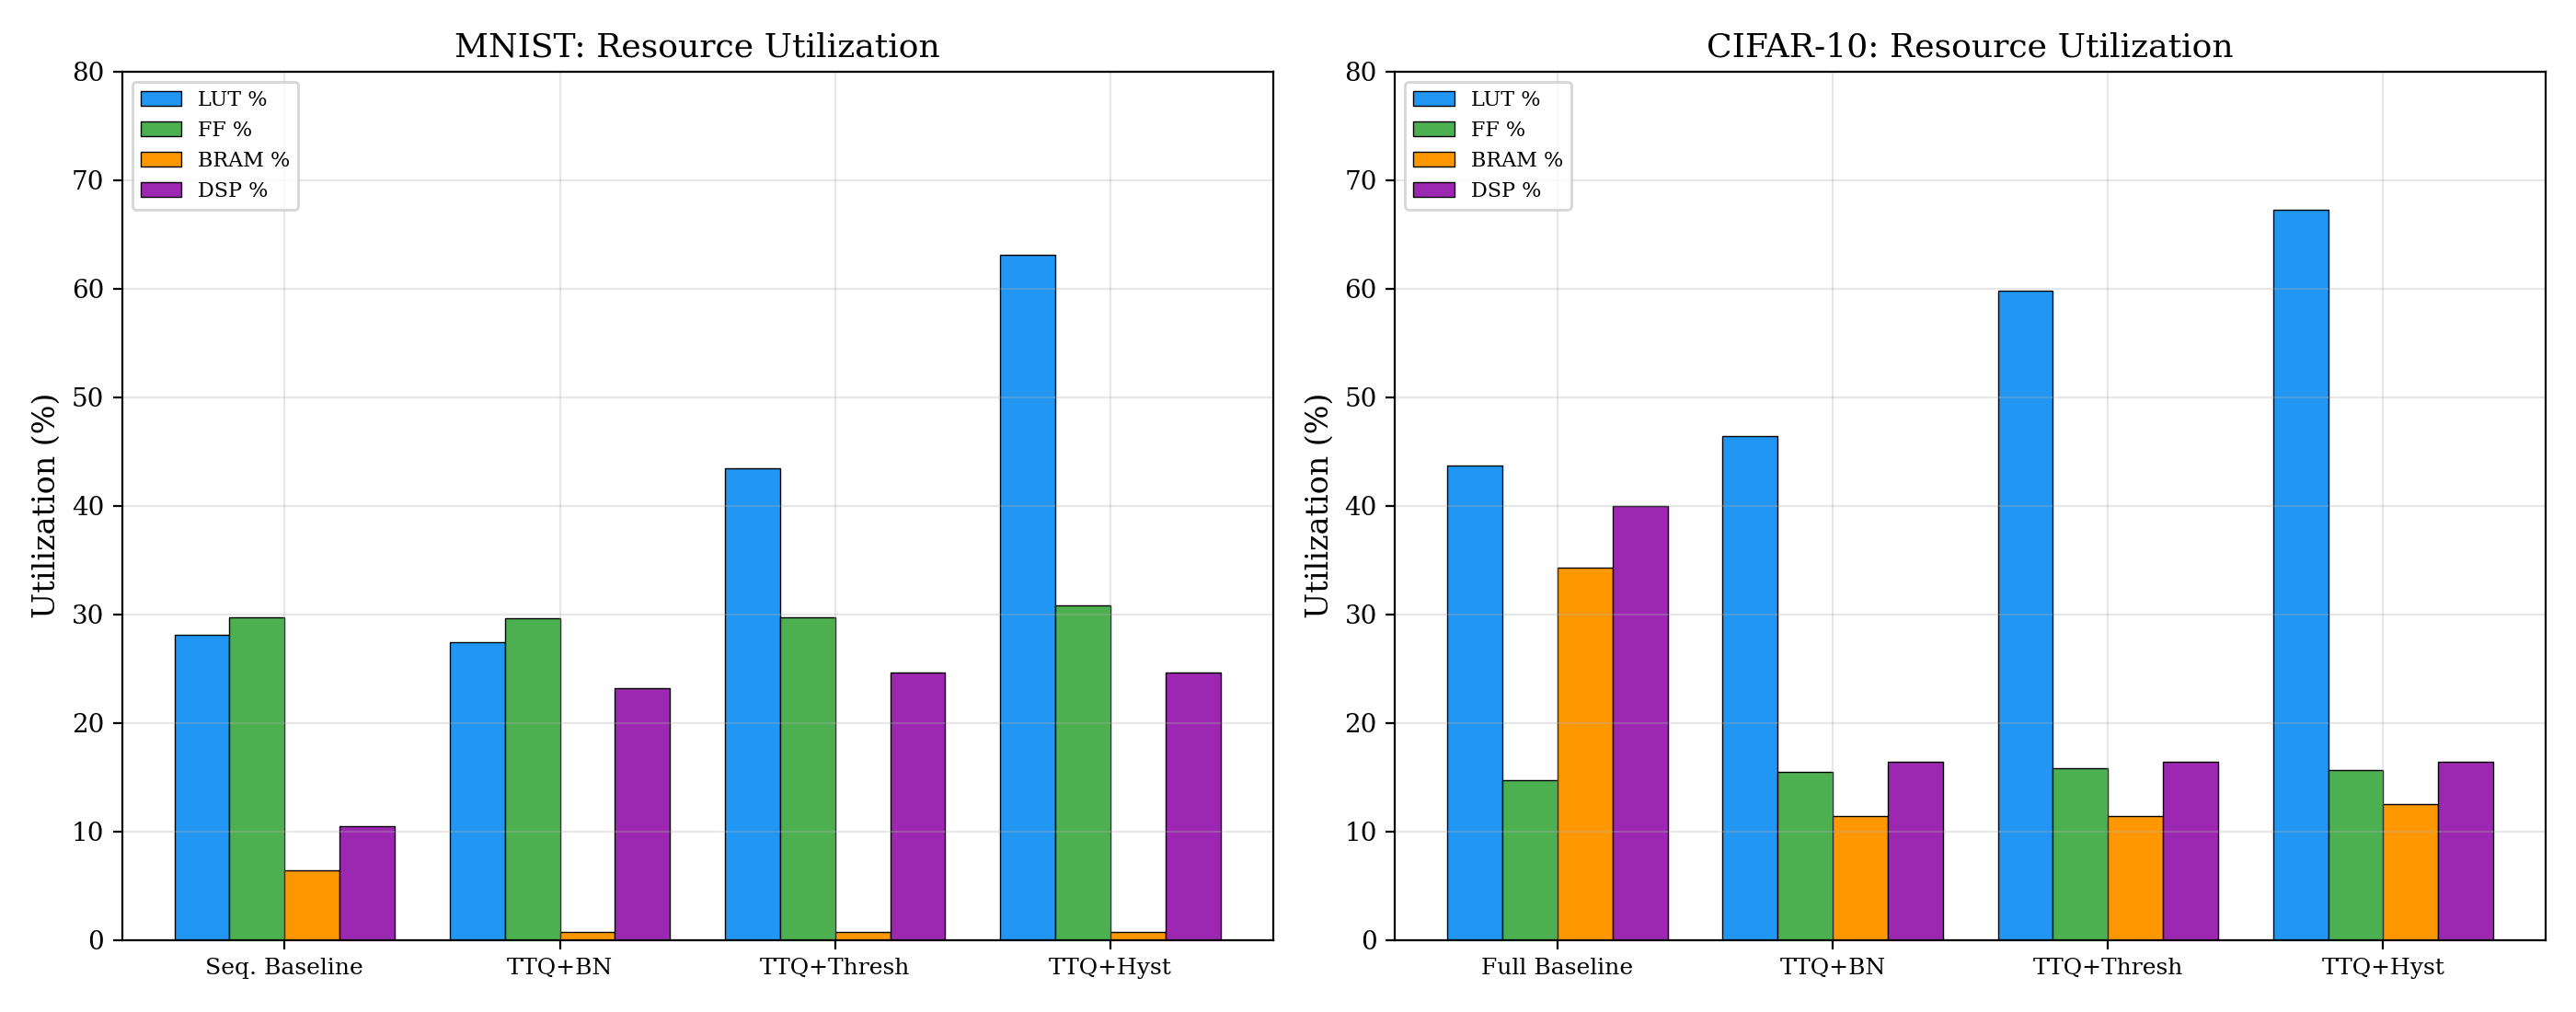
\includegraphics[width=0.48\textwidth]{Images/resource_utilization.png}
\caption{FPGA resource utilization across all designs.}
\label{fig:resources}
\end{figure}

Fig.~\ref{fig:resources} reveals the hardware trade-offs:

\begin{itemize}[nosep]
    \item \textbf{LUT Scaling}: TTQ+BN adds $<$3\% LUT overhead over baselines. Threshold comparators add $\sim$16\%, while hysteresis spatial resolvers add $\sim$20\%, approaching the Zynq-7020's capacity ceiling.
    \item \textbf{BRAM Compression}: TTQ reduces BRAM from 6.4\% to 0.7\% (MNIST) and from 34.3\% to 11.4\% (CIFAR-10) -- directly from $16\times$ weight compression.
    \item \textbf{DSP Redistribution}: On CIFAR-10, TTQ reduces DSPs from 88 (40\%) to 36 (16.4\%) by eliminating per-tap multipliers. On MNIST, DSPs increase (23$\to$51) because the baseline's single shared multiplier was already minimal, while TTQ adds dedicated $W_p/W_n$ scaling multipliers per module.
\end{itemize}

\begin{figure}[H]
\centering
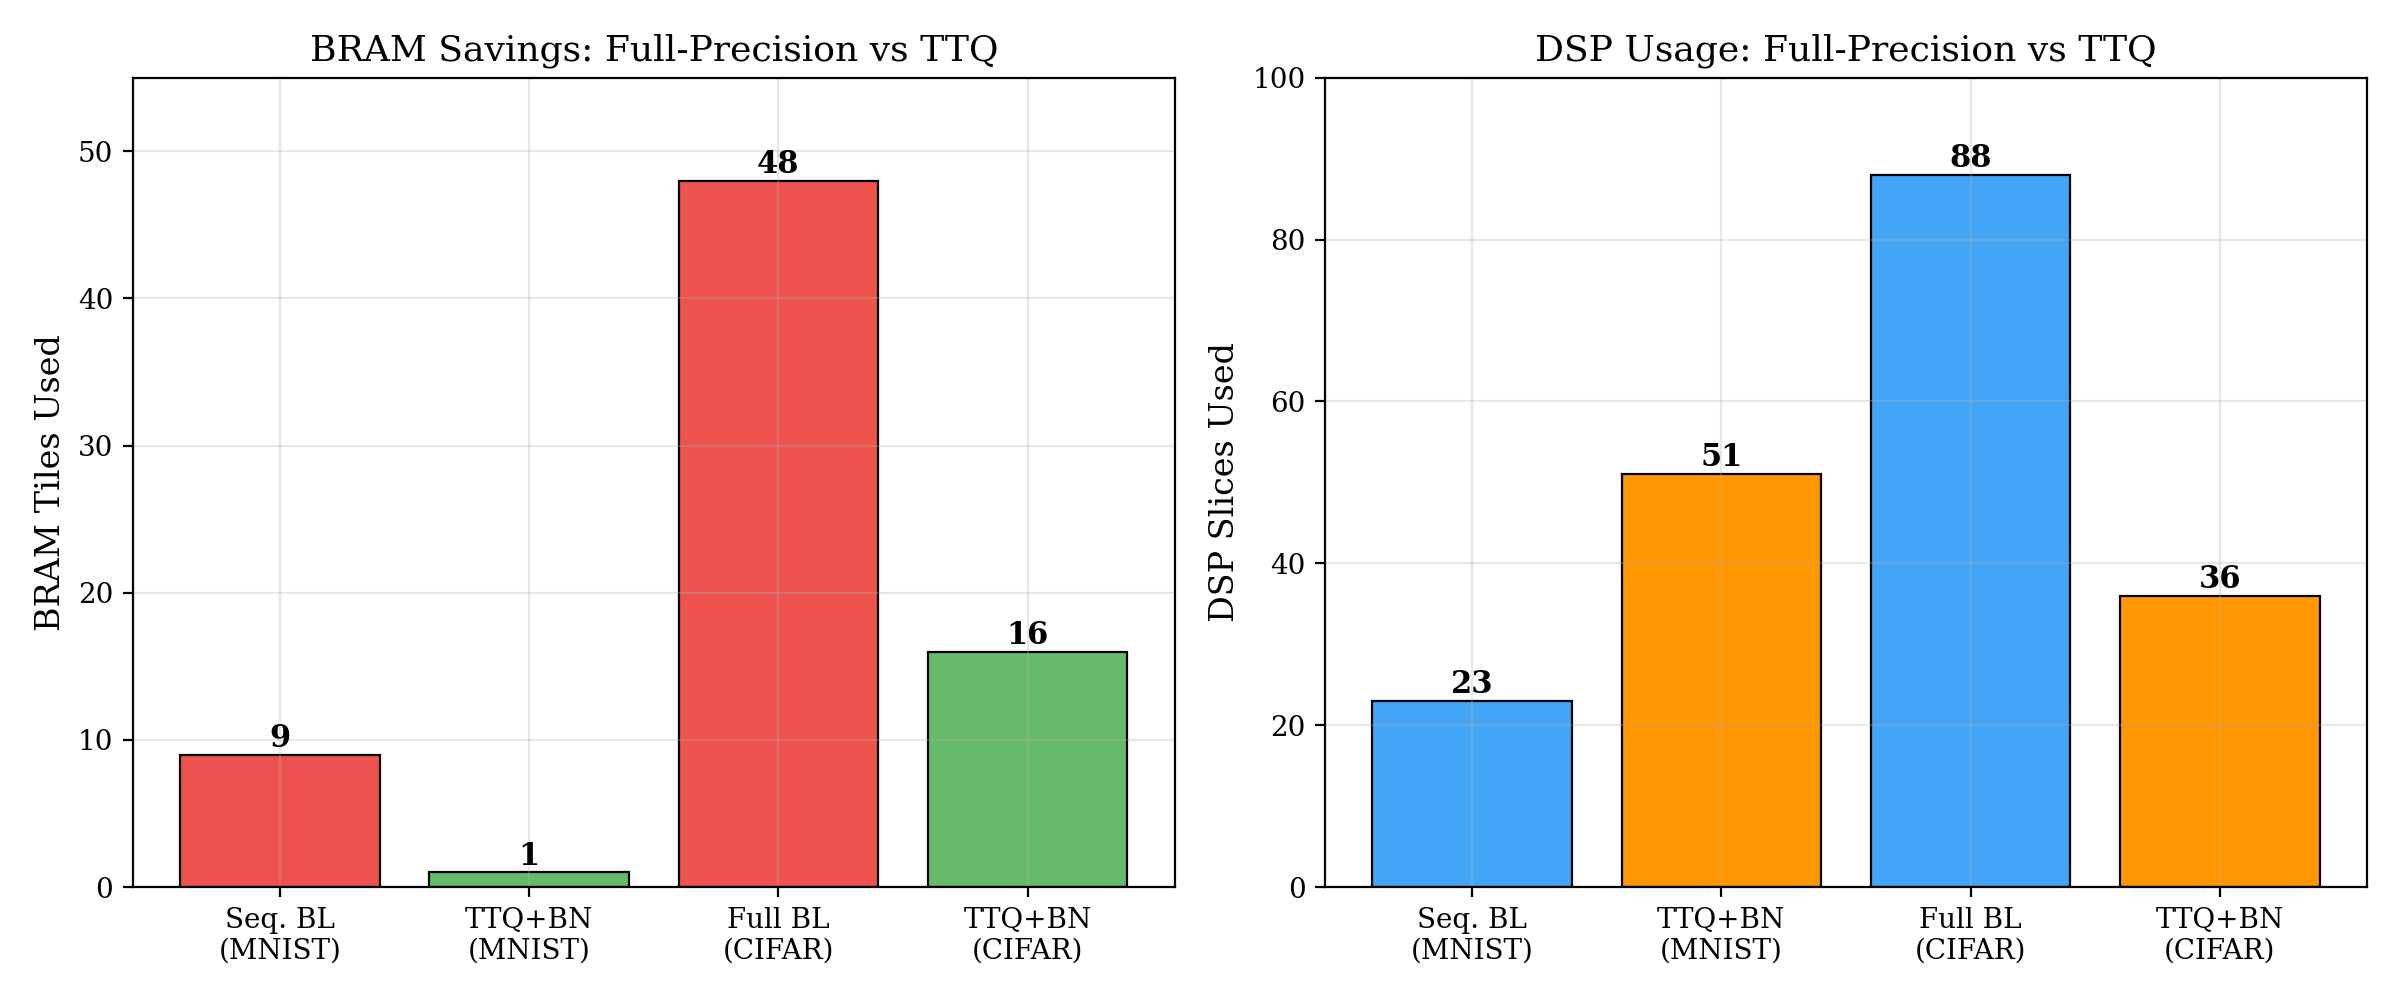
\includegraphics[width=0.48\textwidth]{Images/bram_dsp_comparison.png}
\caption{BRAM and DSP savings from TTQ weight compression.}
\label{fig:bram_dsp}
\end{figure}

\subsection{Latency and Speedup Analysis}

\begin{figure}[H]
\centering
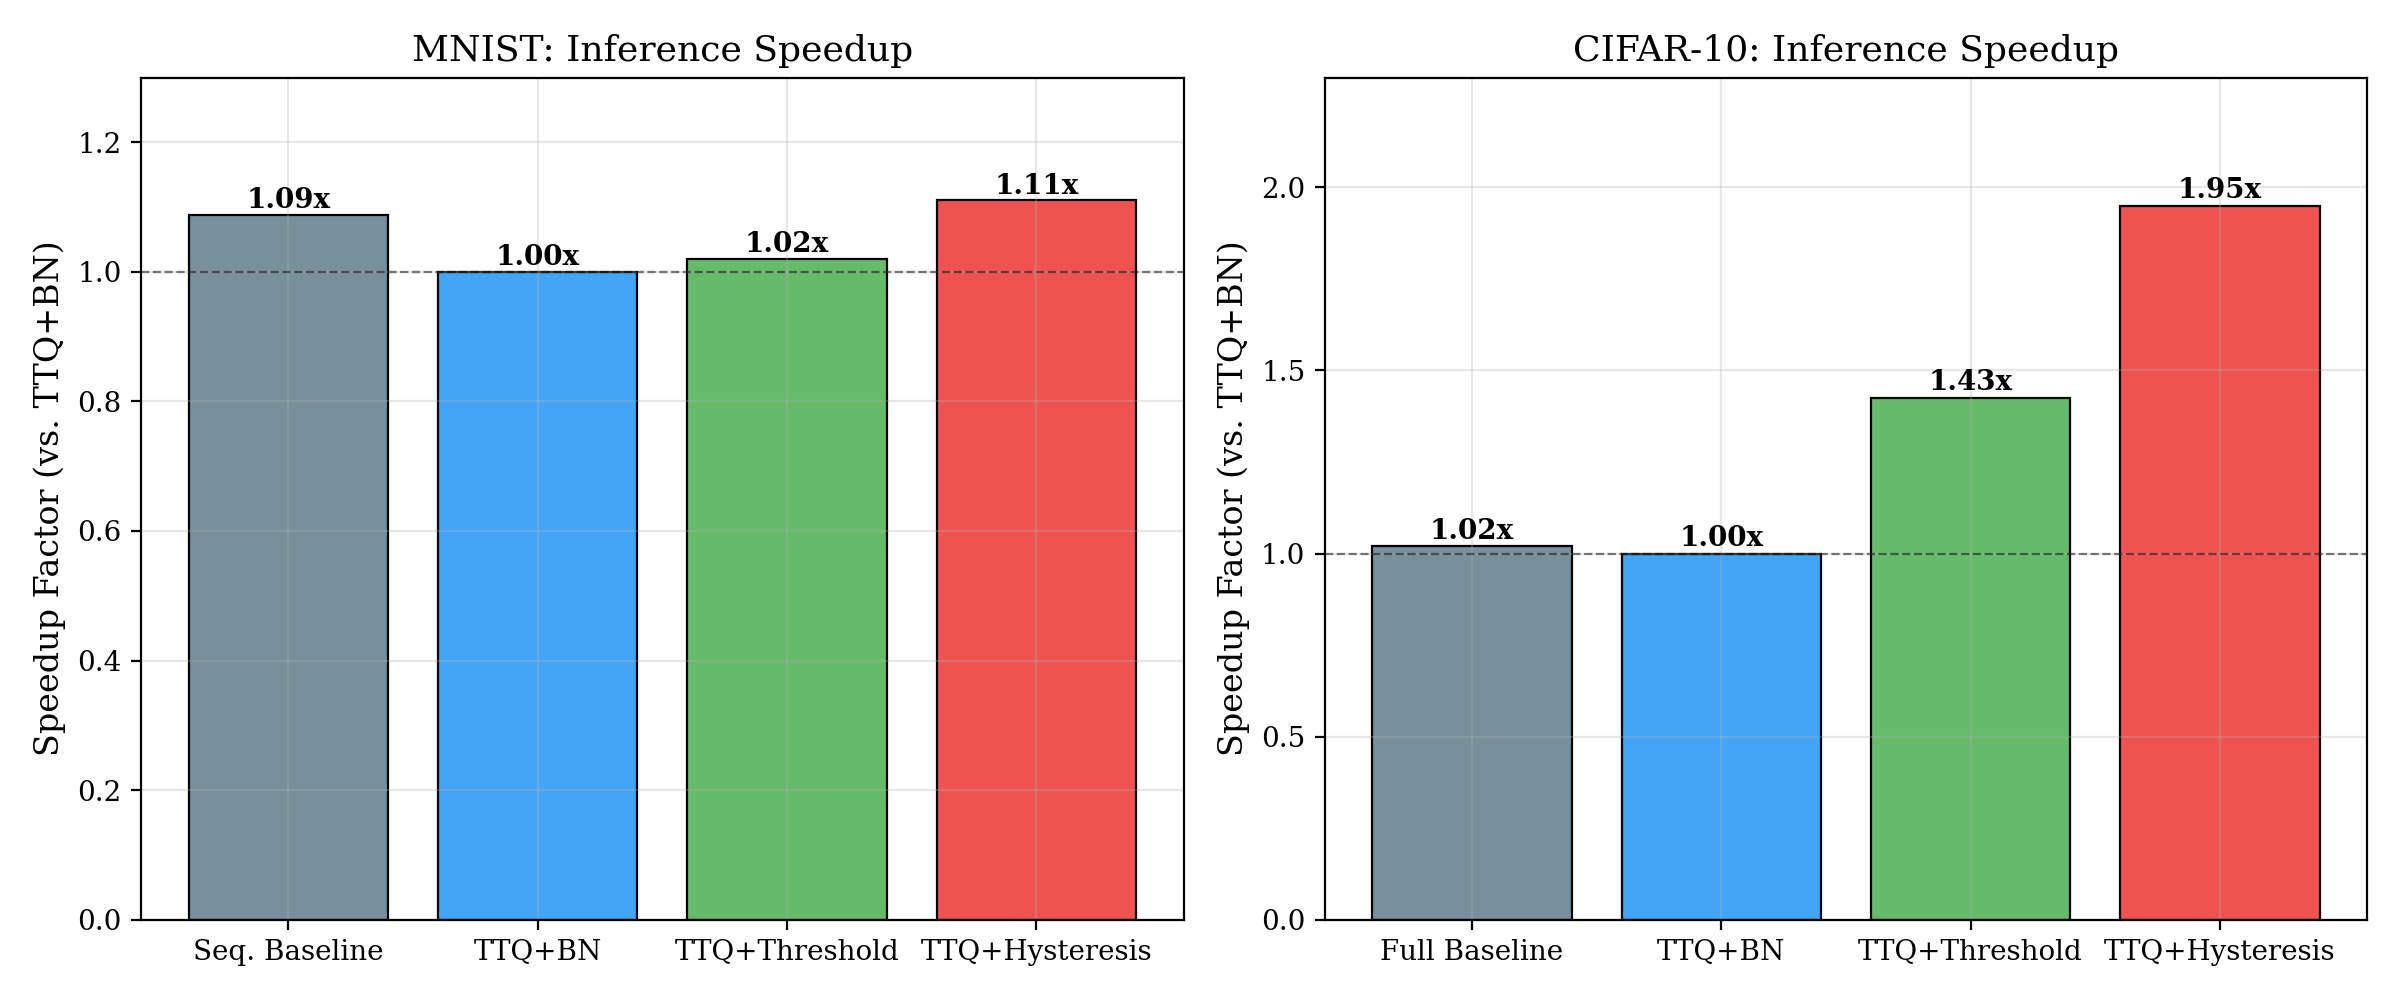
\includegraphics[width=0.48\textwidth]{Images/speedup_comparison.png}
\caption{Inference speedup relative to TTQ+BN baseline.}
\label{fig:speedup}
\end{figure}

Fig.~\ref{fig:speedup} shows speedup factors. On CIFAR-10, the progression from threshold ($1.43\times$) to hysteresis ($1.95\times$) reflects the deeper network's higher natural sparsity in intermediate layers. On MNIST, speedup is modest ($1.02\times$ to $1.11\times$) due to the already-low cycle count.

\subsubsection{CIFAR-10 Per-Layer Cycle Breakdown}

Table~\ref{tab:cifar_layers} decomposes inference cycles by layer.

\begin{table}[H]
\centering
\caption{CIFAR-10 Per-Layer Inference Cycles}
\label{tab:cifar_layers}
\resizebox{\columnwidth}{!}{
\begin{tabular}{lcccc}
\toprule
\textbf{Layer} & \textbf{Active \%} & \textbf{TTQ+BN} & \textbf{+Thresh} & \textbf{+Hyst} \\
\midrule
Conv1+Pool1 & 100\% & 376,834 & 362,130 & 360,594 \\
Mask Gen 1 & -- & -- & -- & 36,973 \\
Conv2+Pool2 & 66.1\% & 1,257,474 & 903,606 & 575,863 \\
Mask Gen 2 & -- & -- & -- & 16,683 \\
Conv3 & 47.0\% & 604,162 & 382,759 & 256,726 \\
Mask Gen 3 & -- & -- & -- & 14,177 \\
Conv4 & 26.3\% & 604,162 & 345,167 & 194,697 \\
GAP & -- & 4,226 & 4,227 & 4,227 \\
FC1+BN & $\sim$60\% & 27,906 & 17,605 & 13,070 \\
FC2 & -- & 3,006 & 2,463 & 2,254 \\
\midrule
\textbf{Total} & & \textbf{2,877,770} & \textbf{2,017,961} & \textbf{1,475,264} \\
\textbf{Speedup} & & 1.00$\times$ & 1.43$\times$ & 1.95$\times$ \\
\bottomrule
\end{tabular}
}
\end{table}

The largest speedup occurs in Conv4 (active ratio: 26.3\%), where hysteresis achieves $3.10\times$ layer-wise speedup. Mask generation overhead (67,833 total cycles) is amortized by 1,470,339 cycles saved in computation.

\begin{figure}[H]
\centering
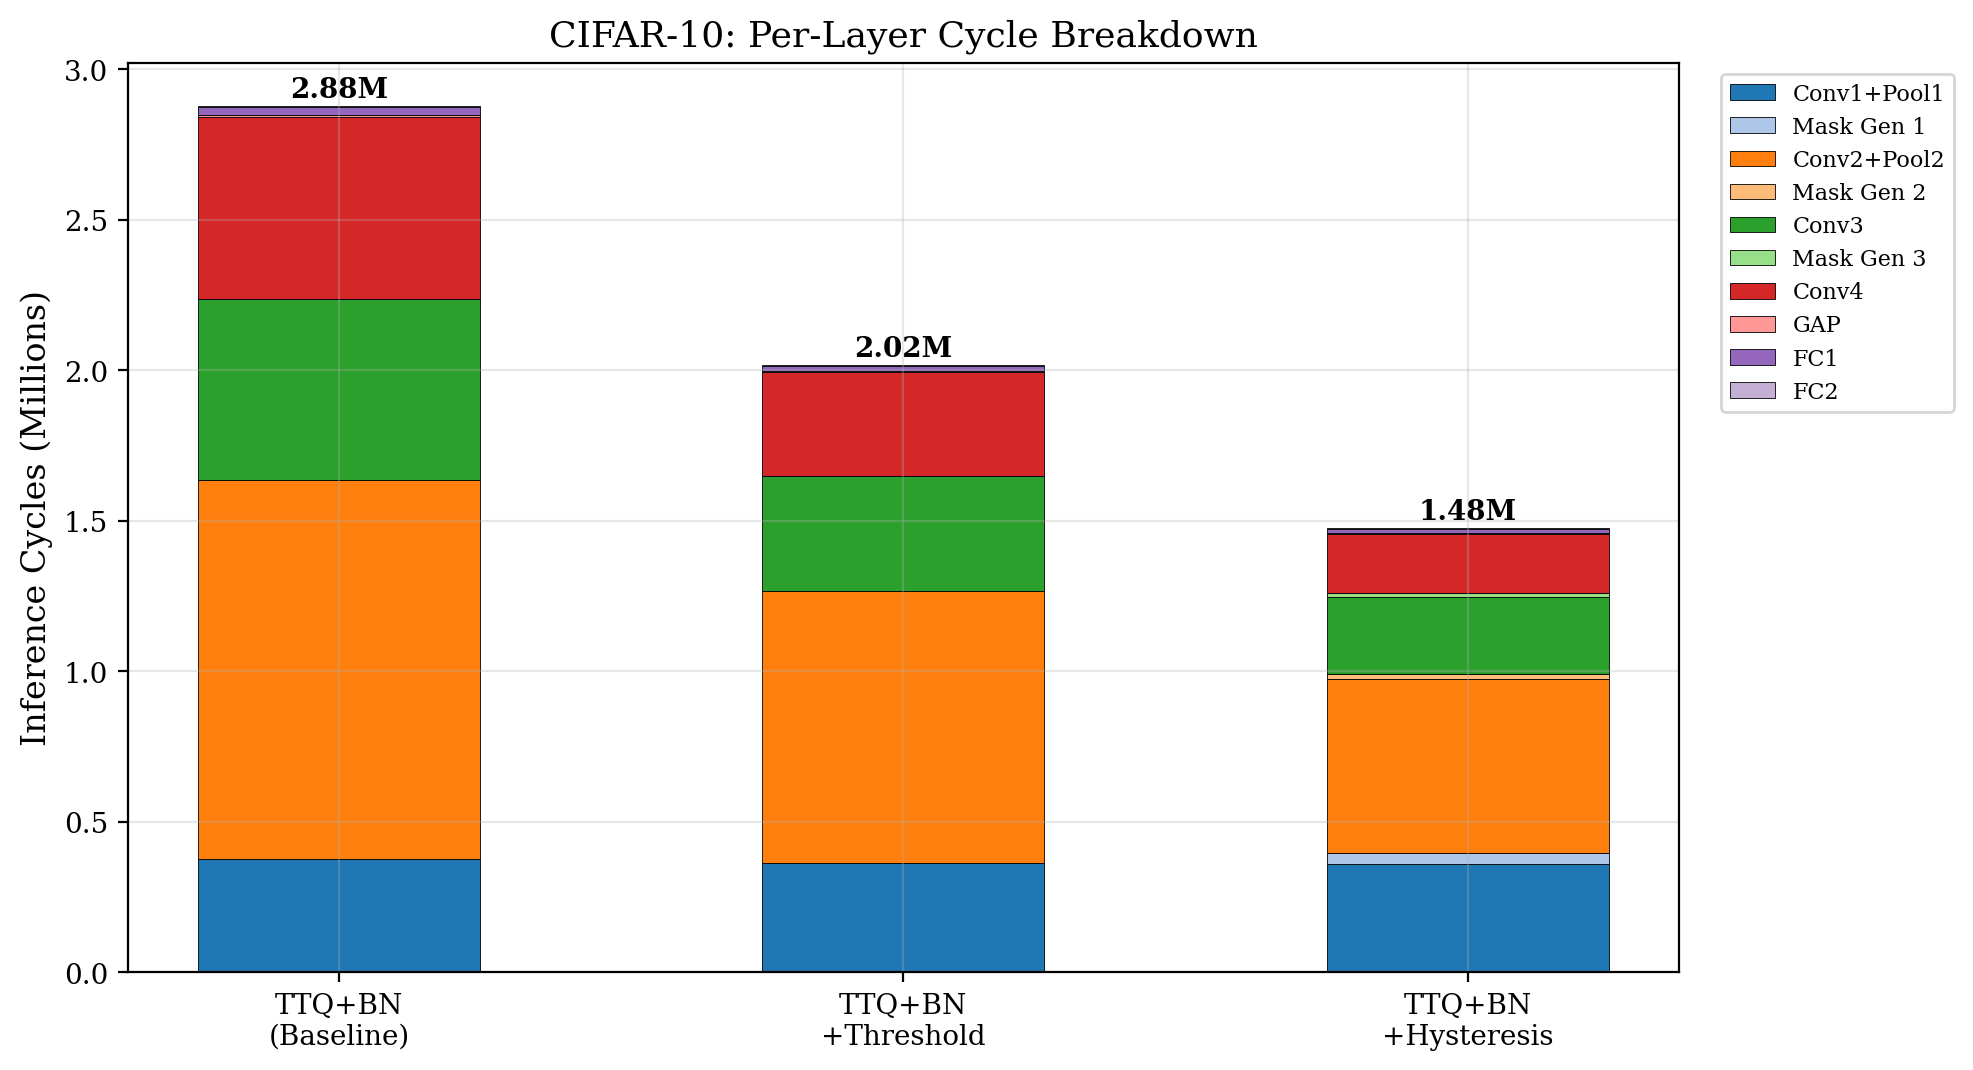
\includegraphics[width=0.48\textwidth]{Images/cifar10_cycle_breakdown.png}
\caption{CIFAR-10 per-layer cycle breakdown (stacked bar).}
\label{fig:cycle_breakdown}
\end{figure}

\subsection{Power and Energy Analysis}

\begin{figure}[H]
\centering
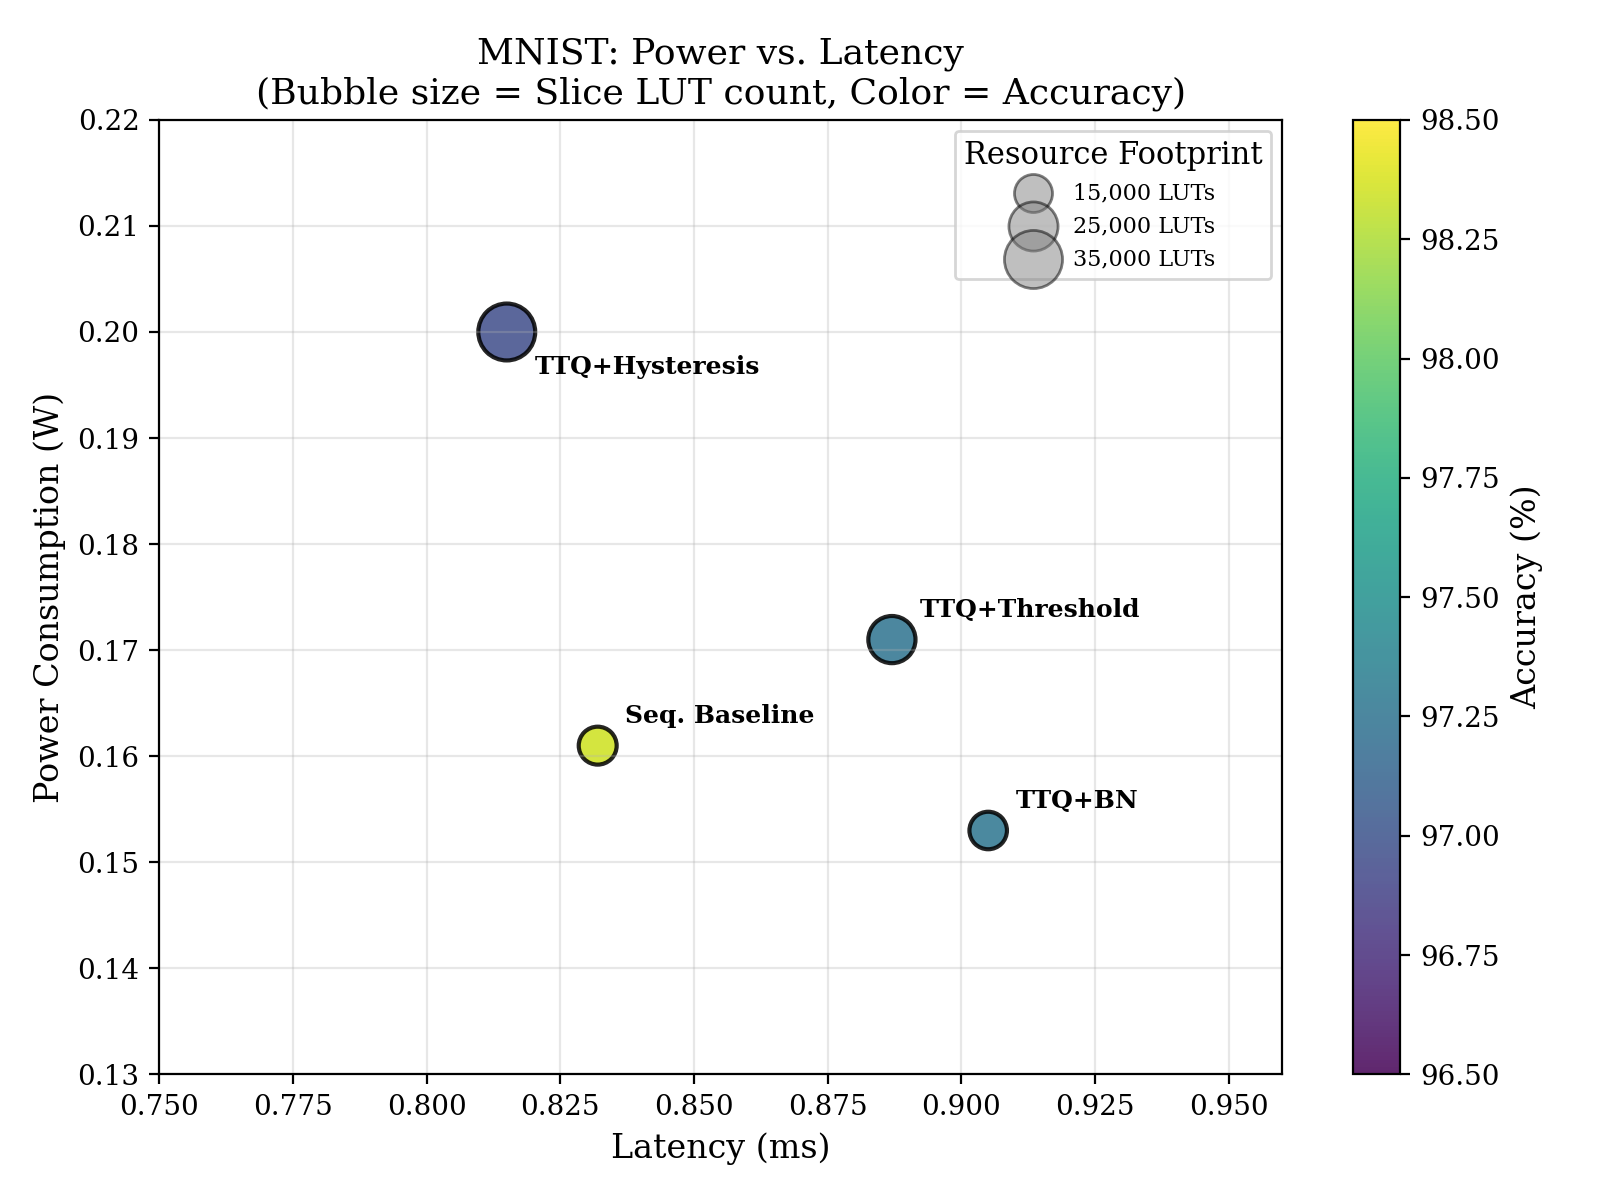
\includegraphics[width=0.48\textwidth]{Images/mnist_power_vs_latency.png}
\caption{MNIST: Power vs. Latency (bubble size = LUT count).}
\label{fig:mnist_pvl}
\end{figure}

\begin{figure}[H]
\centering
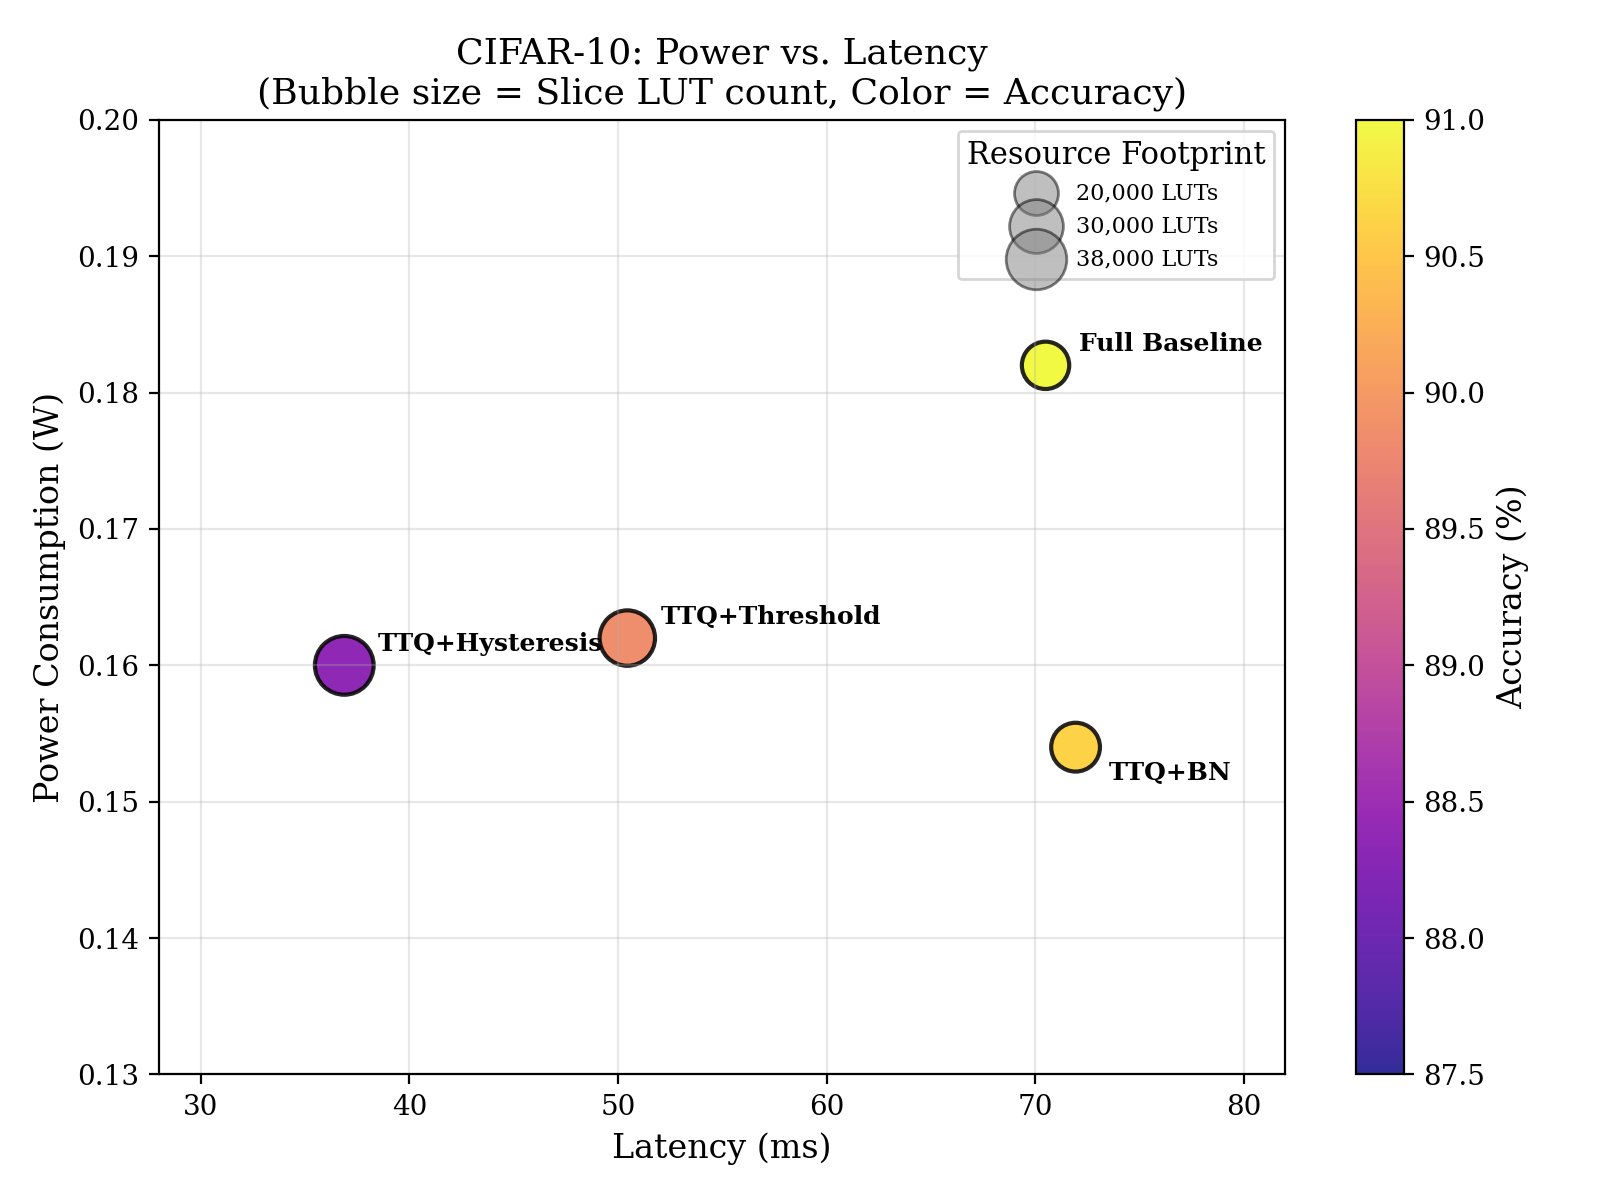
\includegraphics[width=0.48\textwidth]{Images/cifar10_power_vs_latency.png}
\caption{CIFAR-10: Power vs. Latency (bubble size = LUT count).}
\label{fig:cifar_pvl}
\end{figure}

All designs operate at $<$200~mW. Device static power ($\sim$106~mW) dominates, compressing apparent differences. TTQ+BN achieves the lowest dynamic power (0.048~W) due to minimal switching activity from ternary accumulation.

\begin{figure}[H]
\centering
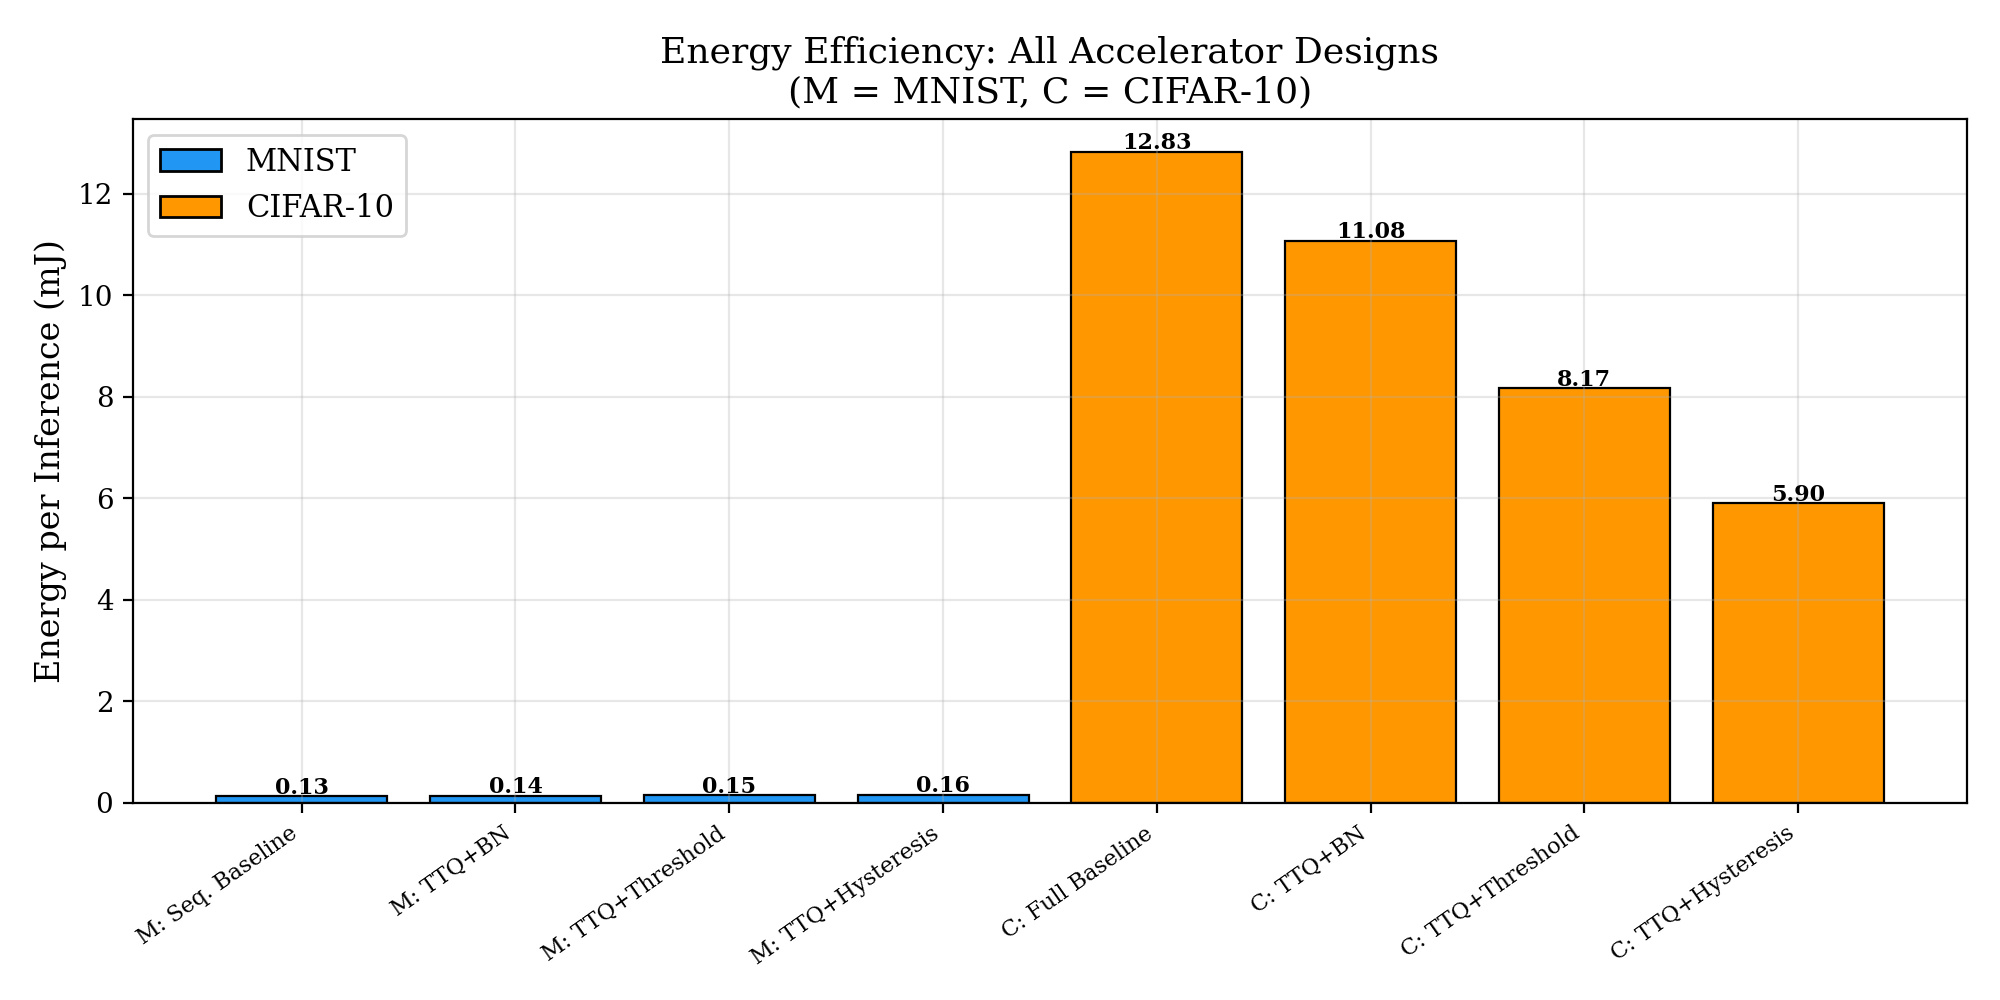
\includegraphics[width=0.48\textwidth]{Images/energy_per_inference.png}
\caption{Energy per inference across all designs.}
\label{fig:energy}
\end{figure}

Fig.~\ref{fig:energy} reveals a critical insight: despite higher instantaneous power, the hysteresis design achieves the lowest energy per inference on CIFAR-10 (5.9~mJ vs. 12.8~mJ for the baseline) because its $1.95\times$ latency reduction more than compensates for the power increase. This demonstrates that latency co-optimization is essential for energy efficiency.

\subsection{Activation Sparsity and Pruning Effectiveness}

\begin{figure}[H]
\centering
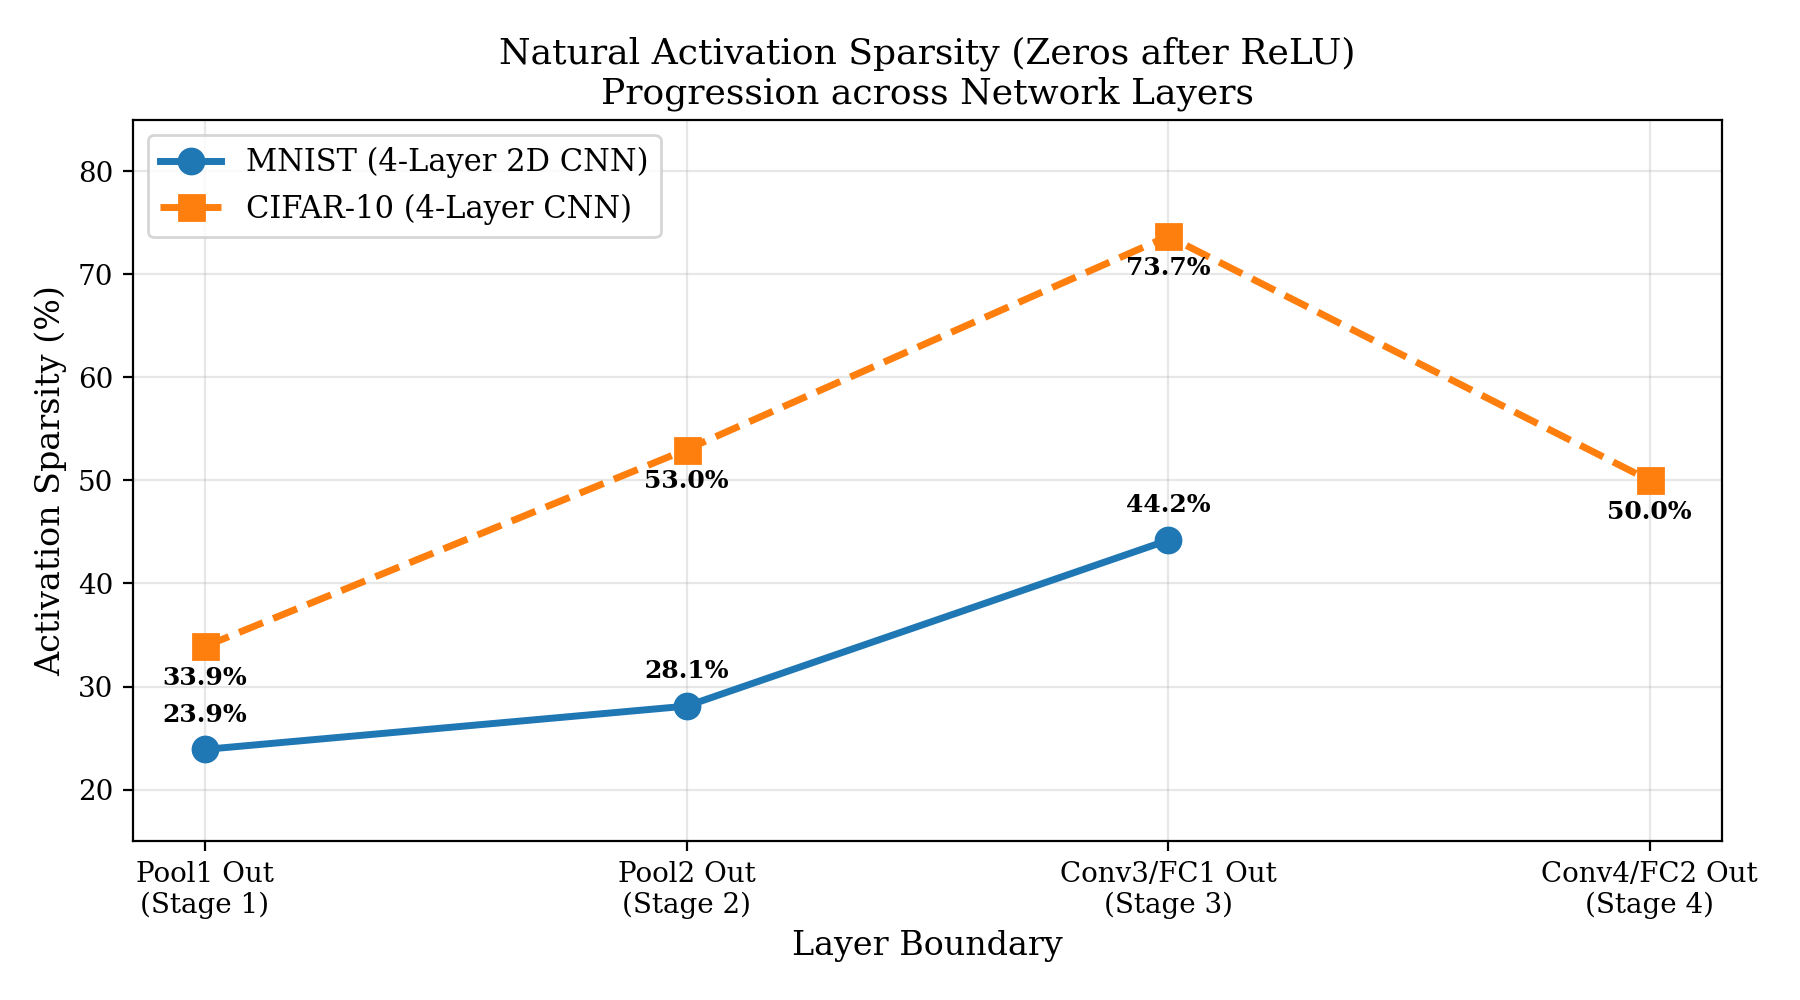
\includegraphics[width=0.48\textwidth]{Images/activation_vs_sparsity.png}
\caption{Natural activation sparsity progression across layers.}
\label{fig:sparsity}
\end{figure}

\begin{figure}[H]
\centering
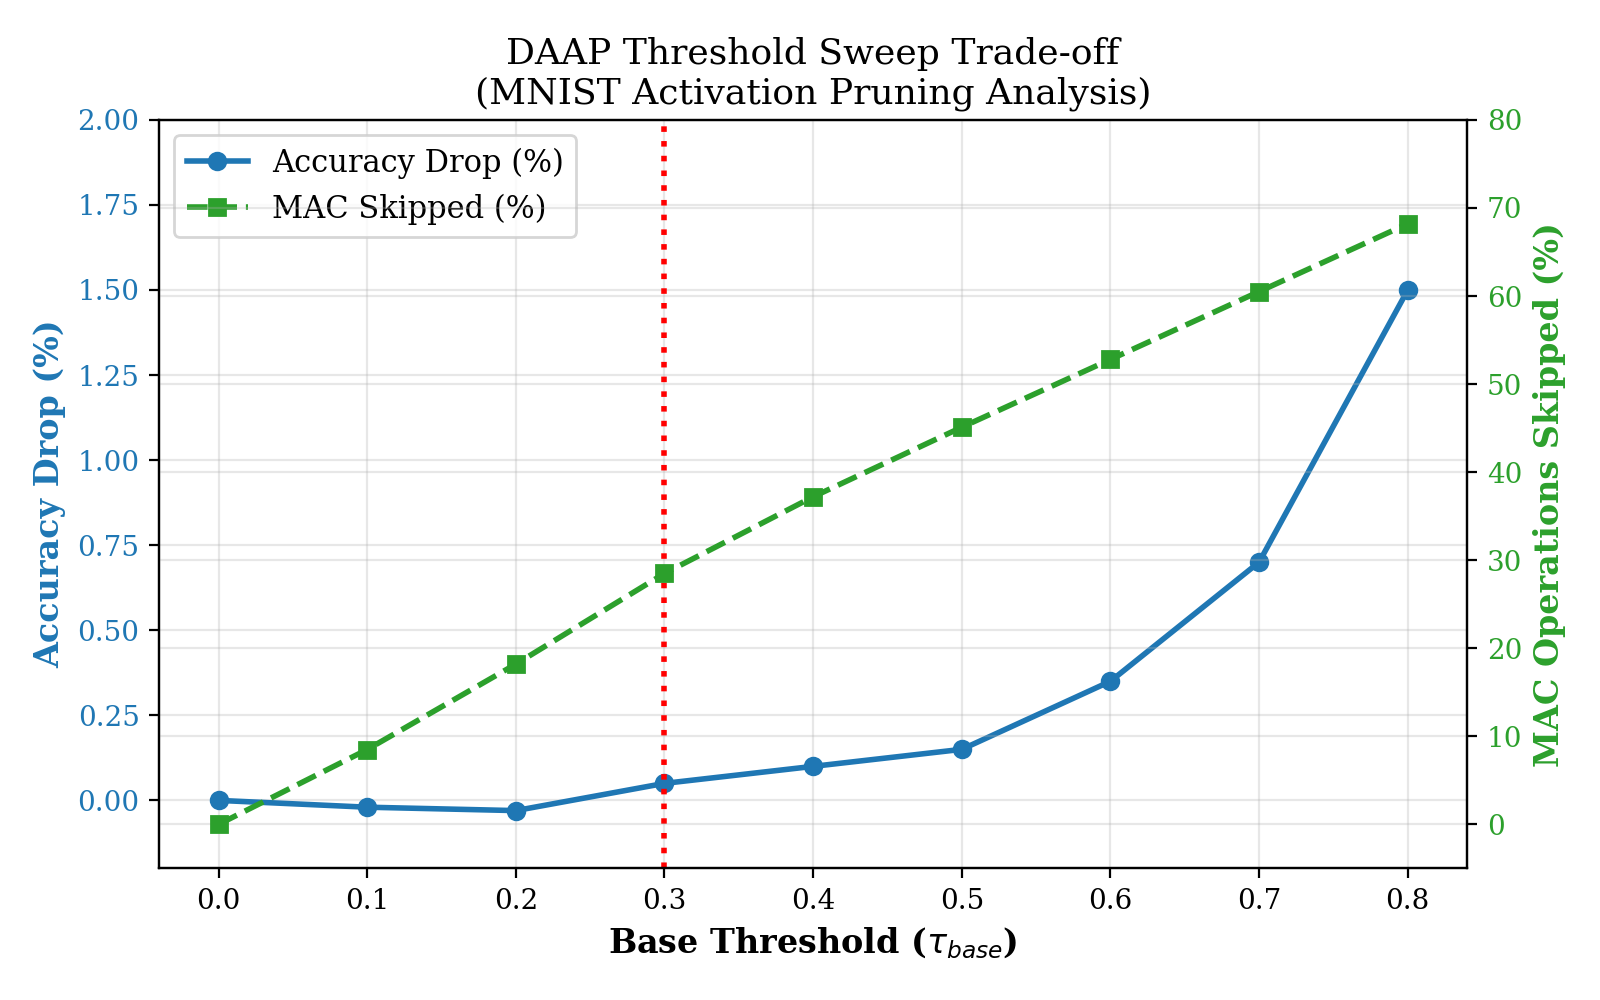
\includegraphics[width=0.48\textwidth]{Images/daap_threshold_sweep.png}
\caption{DAAP threshold sweep: accuracy vs. MAC skip rate.}
\label{fig:daap_sweep}
\end{figure}

Fig.~\ref{fig:sparsity} shows that CIFAR-10 develops up to 73.7\% sparsity in Conv3, while MNIST reaches 44.2\% in FC1. Fig.~\ref{fig:daap_sweep} shows the optimal MNIST threshold at $\tau_{\text{base}}=0.30$, achieving $\sim$28.5\% MAC skip rate with negligible accuracy loss.

\subsection{Timing Closure}

\begin{table}[H]
\centering
\caption{Timing Closure Summary}
\label{tab:timing}
\begin{tabular}{lccc}
\toprule
\textbf{Design} & \textbf{Clock} & \textbf{WNS} & \textbf{WHS} \\
\midrule
MNIST Baseline & 100 MHz & +0.291 ns & +0.116 ns \\
MNIST TTQ+BN & 100 MHz & +0.853 ns & +0.043 ns \\
MNIST TTQ+Thresh & 100 MHz & +0.039 ns & +0.116 ns \\
MNIST TTQ+Hyst & 100 MHz & +0.289 ns & +0.116 ns \\
\midrule
CIFAR Baseline & 40 MHz & +9.472 ns & +0.132 ns \\
CIFAR TTQ+BN & 40 MHz & +10.521 ns & +0.132 ns \\
CIFAR TTQ+Thresh & 40 MHz & +10.315 ns & +0.132 ns \\
CIFAR TTQ+Hyst & 40 MHz & +6.225 ns & +0.132 ns \\
\bottomrule
\end{tabular}
\end{table}

All designs achieve timing closure with zero failing endpoints. The MNIST TTQ+Threshold design has the tightest margin (WNS=+0.039~ns) due to the threshold comparator in the critical path. The CIFAR-10 hysteresis design has a reduced margin (WNS=+6.225~ns, $F_{\text{max}} \approx 53.2$~MHz) from the spatial resolution logic.


% ======================================================================
\section{Conclusion and Future Work}
\label{sec:conclusion}
% ======================================================================

\subsection{Summary of Contributions}

This paper presented a systematic hardware co-design study of three progressive optimization strategies for CNN accelerators on the Xilinx Zynq-7020 FPGA:

\begin{enumerate}[nosep]
    \item \textbf{TTQ + BN Folding}: Achieves $16\times$ weight compression, eliminates per-tap DSP usage, and reduces BRAM by up to $9\times$ with accuracy loss of only 1.07\% (MNIST) and 1.24\% (CIFAR-10). This establishes TTQ as a net-positive optimization for any resource-constrained FPGA accelerator.

    \item \textbf{DAAP Thresholding}: Provides a robust, dataset-agnostic $1.43\times$ speedup on CIFAR-10 with $-0.77\%$ accuracy cost. The per-filter density-adaptive threshold calibration ensures that pruning aggressiveness scales automatically with weight sparsity, making DAAP suitable for general-purpose deployment.

    \item \textbf{Spatial Hysteresis Gating}: Achieves the highest speedup ($1.95\times$, CIFAR-10) and lowest energy per inference (5.9~mJ) by creating contiguous zero-clusters. However, its spatial locality assumption introduces data-dependent accuracy sensitivity ($-2.28\%$ on dense CIFAR-10 textures vs. $-0.32\%$ on sparse MNIST digits), making it best suited for applications with inherently sparse inputs.

    \item \textbf{Lookahead FSM}: The 2-tap/4-tap skip-gating mechanism translates activation sparsity into direct clock-cycle savings without pipeline stalls, achieving up to $3.10\times$ layer-wise speedup in Conv4. The physical timing constraint that limits convolution layers to 2-tap lookahead (due to address wrapping complexity) is a fundamental result applicable to any skip-gating accelerator design.
\end{enumerate}

All eight hardware configurations operate at ultra-low power ($<$200~mW), are timing-closed on silicon, and verified end-to-end, validating the feasibility of deploying quantized, pruned CNN accelerators on resource-constrained edge FPGAs.

\subsection{Industrial Relevance}

The strategies demonstrated in this work address key deployment requirements across multiple industries:

\begin{itemize}[nosep]
    \item \textbf{Autonomous Systems}: Sub-millisecond classification (MNIST) and $\sim$37~ms inference (CIFAR-10 with hysteresis) at $\sim$160~mW enable deployment in power-constrained sensor pods for collision avoidance, traffic sign recognition, and UAV navigation.
    \item \textbf{IoT Edge Nodes}: $16\times$ weight compression enables multiple classification heads on a single FPGA, while activation pruning reduces dynamic power during static scenes.
    \item \textbf{Privacy-Preserving Inference}: On-device processing eliminates the need to transmit raw sensor data to cloud servers.
\end{itemize}

\subsection{Future Work}

\begin{enumerate}[nosep]
    \item \textbf{Mixed-Precision Quantization}: Combining 2-bit TTQ in early layers with 4-bit or 8-bit quantization in accuracy-sensitive later layers to recover the accuracy gap while preserving most compression benefits.
    \item \textbf{Channel-Wise Adaptive Thresholds}: Extending DAAP with per-channel (rather than per-filter) threshold calibration to improve pruning granularity on dense datasets.
    \item \textbf{UltraScale+ Migration}: Scaling to Zynq UltraScale+ (ZU9EG: 600K LUTs, 2,520 DSPs) to enable parallel filter processing with TTQ, targeting $>$10$\times$ throughput for real-time object detection (YOLO-class models).
    \item \textbf{Dynamic Reconfiguration}: Leveraging FPGA partial reconfiguration to switch between DAAP and hysteresis gating at runtime based on input scene complexity.
    \item \textbf{Multi-Network Pipelines}: The BRAM freed by $16\times$ TTQ compression can host multiple independent classification heads (e.g., object detection + lane segmentation) on a single fabric.
\end{enumerate}


% ======================================================================
% REFERENCES
% ======================================================================
\begin{thebibliography}{20}

\bibitem{zhu2017}
C.~Zhu, S.~Han, H.~Mao, and W.~J.~Dally, ``Trained ternary quantization,'' in \emph{Proc. Int. Conf. Learn. Represent. (ICLR)}, 2017.

\bibitem{li2016}
F.~Li and B.~Liu, ``Ternary weight networks,'' \emph{arXiv preprint arXiv:1605.04711}, 2016.

\bibitem{courbariaux2016}
M.~Courbariaux, I.~Hubara, D.~Soudry, R.~El-Yaniv, and Y.~Bengio, ``Binarized neural networks,'' in \emph{Proc. Adv. Neural Inf. Process. Syst. (NeurIPS)}, vol.~29, 2016.

\bibitem{han2016}
S.~Han, H.~Mao, and W.~J.~Dally, ``Deep compression: Compressing deep neural networks with pruning, trained quantization and Huffman coding,'' in \emph{Proc. Int. Conf. Learn. Represent. (ICLR)}, 2016.

\bibitem{jacob2018}
B.~Jacob \emph{et al.}, ``Quantization and training of neural networks for efficient integer-arithmetic-only inference,'' in \emph{Proc. IEEE/CVF Conf. Comput. Vis. Pattern Recognit. (CVPR)}, 2018, pp.~2704--2713.

\bibitem{nagel2021}
M.~Nagel, M.~Fournarakis, R.~A.~Amjad, Y.~Bondarenko, M.~van Baalen, and T.~Blankevoort, ``A white paper on neural network quantization,'' \emph{arXiv preprint arXiv:2106.08295}, 2021.

\bibitem{umuroglu2017}
Y.~Umuroglu \emph{et al.}, ``FINN: A framework for fast, scalable binarized neural network inference,'' in \emph{Proc. ACM/SIGDA Int. Symp. Field-Program. Gate Arrays (FPGA)}, 2017, pp.~65--74.

\bibitem{blott2018}
M.~Blott \emph{et al.}, ``FINN-R: An end-to-end deep-learning framework for fast exploration of quantized neural networks,'' \emph{ACM Trans. Reconfig. Technol. Syst.}, vol.~11, no.~3, pp.~1--23, 2018.

\bibitem{venieris2018}
S.~I.~Venieris and C.-S.~Bouganis, ``fpgaConvNet: Mapping regular and irregular convolutions on FPGAs,'' \emph{IEEE Trans. Neural Netw. Learn. Syst.}, vol.~30, no.~2, pp.~326--342, Feb.~2019.

\bibitem{qiu2016}
J.~Qiu \emph{et al.}, ``Going deeper with embedded FPGA platform for convolutional neural network,'' in \emph{Proc. ACM/SIGDA Int. Symp. Field-Program. Gate Arrays (FPGA)}, 2016, pp.~26--35.

\bibitem{sharma2018}
H.~Sharma \emph{et al.}, ``Bit Fusion: Bit-level dynamically composable architecture for accelerating deep neural networks,'' in \emph{Proc. ACM/IEEE Int. Symp. Comput. Archit. (ISCA)}, 2018, pp.~764--775.

\bibitem{albericio2016}
J.~Albericio, P.~Judd, T.~Hetherington, T.~Aamodt, N.~E.~Jerger, and A.~Moshovos, ``Cnvlutin: Ineffectual-neuron-free deep neural network computing,'' in \emph{Proc. ACM/IEEE Int. Symp. Comput. Archit. (ISCA)}, 2016, pp.~1--13.

\bibitem{guo2017}
Y.~Guo, A.~Yao, and Y.~Chen, ``Dynamic network surgery for efficient DNNs,'' in \emph{Proc. Adv. Neural Inf. Process. Syst. (NeurIPS)}, vol.~29, 2016.

\bibitem{guo2019}
K.~Guo \emph{et al.}, ``A survey of FPGA-based neural network inference accelerators,'' \emph{ACM Trans. Reconfig. Technol. Syst.}, vol.~12, no.~1, pp.~1--26, 2019.

\bibitem{wang2019}
E.~Wang, J.~J.~Davis, P.~Y.~K.~Cheung, and G.~A.~Constantinides, ``LUTNet: Learning FPGA configurations for highly efficient neural network inference,'' \emph{IEEE Trans. Comput.}, vol.~69, no.~8, pp.~1228--1241, Aug.~2020.

\bibitem{xilinx_zynq}
AMD/Xilinx, ``Zynq-7000 SoC Technical Reference Manual,'' UG585 (v1.14), 2023.

\bibitem{lecun1998}
Y.~LeCun, L.~Bottou, Y.~Bengio, and P.~Haffner, ``Gradient-based learning applied to document recognition,'' \emph{Proc. IEEE}, vol.~86, no.~11, pp.~2278--2324, Nov.~1998.

\bibitem{krizhevsky2009}
A.~Krizhevsky, ``Learning multiple layers of features from tiny images,'' \emph{Tech. Rep.}, University of Toronto, 2009.

\bibitem{zhang2022}
Y.~Zhang, H.~Zhao, and J.~Gao, ``Structured pruning for efficient neural network acceleration on FPGA,'' in \emph{Proc. IEEE Int. Conf. Field-Program. Logic Appl. (FPL)}, 2022, pp.~1--8.

\bibitem{chen2019}
Y.-H.~Chen, T.~Krishna, J.~S.~Emer, and V.~Sze, ``Eyeriss v2: A flexible accelerator for emerging deep neural networks on mobile devices,'' \emph{IEEE J. Emerg. Sel. Topics Circuits Syst.}, vol.~9, no.~2, pp.~292--308, Jun.~2019.

\end{thebibliography}

\end{document}
